\documentclass[IB]{TFUOC}%IB: CASTELLANO, CAT: CATALÁN, ENG: ANGLÈS
\usepackage{csquotes}
\usepackage{amsmath}
\usepackage[style=numeric, backend=biber]{biblatex}
\addbibresource{referencias.bib} % OBLIGATORIO incluir la extensión .bib
%\usepackage[table]{xcolor}
\usepackage{array}
\usepackage{float}
\usepackage{hyperref}
\definecolor{uocnavy}{RGB}{0, 0, 120}

%Introducción de datos del trabajo
\title{Diseño y evaluación experimental de un esquema de esteganografía de clave pública resistente a compresión JPEG}
\titcrt{Esteganografía de Clave Pública Robusta} %Título corto que aparecerá a la cabecera
\author{Diego Alejandro Higuita Grisales}
\date{03 de Noviembre de 2026}


\nomPDC{Daniel Lerch Hostalot}
% \nomPRA{Daniel Lerch Hostalot}
\titulac{Máster en Ciberseguridad y Privacidad}
\area{\small Protocolos criptográficos y aplicaciones de seguridad}
\idioma{Castellano}
\credits{15}
\parcla{Esteganografía de clave pública, Canal encubierto, Compresión JPEG, QIM, Reed-Solomon, Esteganálisis, Python}
\licenc{ccBy}
%Posibles licencias
%ccByNcNd
%ccByNcSa
%ccByNc
%ccByNd
%ccBySa
%ccBy
%GNU
%copyright


%%%%%%%%%%
% Resumen en el idioma

\abstractidioma{
En el presente Trabajo Final de Máster vamos a abordar el diseño, implementación y evaluación experimental de un sistema de esteganografía de clave pública en el dominio transformado. El objetivo principal es estudiar la viabilidad de transmitir una trama experimental de 32 bits —concebida como señalización experimental— a través de imágenes digitales expuestas a un canal con pérdida por recompresión JPEG. Se adopta como modelo de amenaza una comunicación bajo observación o censura, con un emisor (\textit{Alice}), un receptor (\textit{Bob}) y un observador (\textit{warden}) que puede analizar las imágenes o recomprimirlas. El sistema utiliza las imágenes de cobertura como medio de transporte encubierto y vincula el mapa de posiciones de inserción a la clave privada del receptor mediante X25519 y HKDF. La metodología propuesta combina la modulación por índice de cuantificación (QIM) sobre coeficientes de la Transformada Discreta del Coseno (DCT) con la codificación de canal Reed--Solomon para corregir errores de extracción dentro de la capacidad correctora del código. La evaluación del prototipo analiza el compromiso entre la fiabilidad en la extracción del mensaje, la degradación visual de la estego-imagen ($\mathrm{PSNR}$ y $\mathrm{SSIM}$) y la detectabilidad estadística mediante la suite de estegoanálisis Aletheia. Los resultados obtenidos en laboratorio permiten caracterizar el comportamiento y las limitaciones de la inserción frecuencial para el establecimiento de canales encubiertos en entornos con compresión de imagen.
}

% Resumen en inglés.
\abstractenglish{
In this Master's Thesis, we address the design, implementation, and experimental evaluation of a public-key steganography system in the transform domain. The main objective is to investigate the feasibility of transmitting a 32-bit experimental frame, used as experimental signaling, through digital images exposed to a lossy channel caused by JPEG recompression. The threat model is a communication under surveillance or censorship, with a sender (\textit{Alice}), a receiver (\textit{Bob}) and a warden that may analyze or recompress the images. The system uses cover images as a covert medium and ties the embedding position map to the receiver's private key through X25519 and HKDF. The proposed methodology combines Quantization Index Modulation (QIM) applied to Discrete Cosine Transform (DCT) coefficients with Reed--Solomon channel coding to correct extraction errors within the error-correction capability of the code. The prototype evaluation examines the trade-off between message extraction reliability, stego-image visual degradation ($\mathrm{PSNR}$ and $\mathrm{SSIM}$), and statistical detectability using the Aletheia steganalysis framework. The laboratory results characterize the behavior and limitations of frequency-domain embedding for establishing covert channels in image-compression environments.
}

\begin{document}

\estructura

\tableofcontents
\newpage
\begingroup
\let\clearpage\relax
\listoffigures
\listoftables
\endgroup




\chapter{Introducción}

El presente Trabajo Final de Máster se enmarca en el estudio experimental de la esteganografía de clave pública en imágenes digitales frente a canales con pérdida. En este primer capítulo establecemos el marco general del proyecto; analizamos el contexto conceptual y la problemática técnica, detallamos los objetivos generales y específicos, definimos la metodología de trabajo y presentamos la planificación temporal prevista para el desarrollo del prototipo y su evaluación.

\section{Contexto y justificación del trabajo}
\label{sec:contexto_justificacion}

\subsection{Motivación y Modelo de Amenaza}
En determinados escenarios de comunicación sometidos a observación o supervisión masiva, la criptografía convencional no resuelve por sí sola el problema de ocultar la existencia de un intercambio de información. Aunque el cifrado protege la confidencialidad del contenido, la presencia de un flujo de datos cifrados resulta explícitamente visible para un observador externo, revelando la intención de mantener una comunicación secreta \cite{5,8}.

Desde esta perspectiva, la esteganografía nos ofrece un enfoque complementario: en lugar de limitarse a proteger el contenido de un mensaje, busca integrarlo en un elemento portador aparentemente inocuo, como por ejemplo una imagen digital, con el propósito de reducir los indicios de que la comunicación se está produciendo \cite{5}. 

En este trabajo adoptamos el modelo conceptual clásico de comunicación entre dos partes legítimas, \textit{Alice} (emisora) y \textit{Bob} (receptor), bajo la supervisión de un observador denominado \textit{warden}. \textit{Alice} genera una imagen portadora que contiene una señal experimental destinada a \textit{Bob}. El receptor dispone de una clave privada ($SK_B$) que, junto con la información pública necesaria del protocolo (su clave pública $PK_B$ y la clave pública efímera de \textit{Alice}), le permite derivar, mediante ECDH/X25519, HKDF y un generador pseudoaleatorio (PRNG), el mapa secreto de posiciones utilizado durante la inserción. Por su parte, consideramos dos posibles capacidades del \textit{warden}: en un escenario pasivo, analiza las imágenes mediante técnicas de estegoanálisis para intentar identificar la presencia de modificaciones esteganográficas; en un escenario activo, puede aplicar transformaciones sobre ellas, como la recompresión JPEG con pérdida, que podrían degradar la señal transmitida.

La esteganografía de clave pública traslada la asimetría criptográfica a los canales encubiertos. Aunque la teoría de la información estricta impide este esquema sin un secreto previo compartido, von Ahn y Hopper demostraron su viabilidad bajo supuestos de seguridad computacional \cite{4}. En este modelo, \textit{Alice} utiliza la clave pública de \textit{Bob} ($PK_B$) para generar el soporte esteganográfico. La capacidad para reconstruir el mapa secreto de posiciones y acceder al contenido oculto queda vinculada a la disponibilidad de la clave privada del receptor ($SK_B$) \cite{4} y de la información pública necesaria para el protocolo. De este modo, bajo los supuestos criptográficos del mecanismo empleado, el conocimiento del algoritmo y de la información pública no debería permitir a un tercero reconstruir el mapa secreto sin disponer de la clave privada correspondiente.

\subsection{Entorno Experimental y Definición de la Trama}
A partir de este marco, en el presente trabajo estudiamos la viabilidad de un canal de señalización encubierta sobre imágenes digitales sometidas a recompresión JPEG con pérdida. El proyecto se desarrolla íntegramente en un entorno experimental controlado, utilizando un conjunto de imágenes de prueba y transformaciones reproducibles, sin contemplar su uso en entornos reales ni la transmisión de información operativa.

Para evaluar de forma cuantitativa la fiabilidad del canal, el vector de información (\textit{payload}) se restringe a una trama sintética compacta de 32 bits ($M$):
\begin{equation}
M = V \parallel T
\end{equation}
donde $V$ representa un campo de 8 bits destinado al identificador de versión del protocolo y $T$ corresponde a un patrón numérico sintético de 24 bits:
\begin{equation}
|M| = |V| + |T| = 8 + 24 = 32\,\text{bits}
\end{equation}

Esta trama cumple una función exclusivamente experimental: el patrón $T$ se emplea únicamente para medir la tasa de error de bit ($\mathrm{BER}$) mediante comparación bit a bit entre la señal emitida y la extraída, y nunca para verificar la integridad del mensaje. Se declara explícitamente que el prototipo no incluye autenticación de origen, firmas digitales, $\mathrm{MAC}$ ni comprobación de integridad. Esta decisión nos permite acotar el alcance del prototipo y mantener la trama centrada en la evaluación experimental de la transmisión y recuperación de información. Asimismo, el sistema opera exclusivamente sobre la componente de luminancia ($Y$) del espacio de color YCbCr y solo evalúa la degradación por recompresión JPEG, sin considerar ataques geométricos.

\subsection{El Desafío del Canal Frecuencial JPEG}
El canal de transmisión frecuencial presenta un desafío técnico crítico. La compresión JPEG divide la imagen en bloques de $8 \times 8$ píxeles y aplica la Transformada Discreta del Coseno (DCT), cuantificando los coeficientes resultantes y provocando una pérdida irreversible de información \cite{10}. Este proceso puede alterar o eliminar las modificaciones realizadas mediante métodos esteganográficos elementales del dominio espacial, como la modificación del bit menos significativo (LSB) \cite{3}.

Para estudiar la resistencia frente a esta degradación, planteamos una técnica de inserción en el dominio frecuencial que combina la modulación por índice de cuantificación (\textit{Quantization Index Modulation}, QIM)\cite{11} sobre coeficientes DCT seleccionados con un código de corrección de errores Reed--Solomon $RS(8,4)$ \cite{reed1960}. QIM permite representar los bits mediante regiones de decisión definidas sobre los coeficientes, con el propósito de tolerar determinadas perturbaciones introducidas por la recompresión. Por su parte, Reed--Solomon incorpora redundancia para corregir errores en los símbolos recibidos, dentro de la capacidad correctora de la configuración utilizada. La eficacia de esta combinación frente a JPEG deberá determinarse experimentalmente.

La evaluación experimental caracterizará la relación entre la fiabilidad en la extracción ($\mathrm{BER}$), la calidad visual ($\mathrm{PSNR}$, $\mathrm{SSIM}$) y la detectabilidad estadística frente a la suite de estegoanálisis Aletheia \cite{1}.

\section{Objetivos y alcance del trabajo}
\label{sec:objetivos_alcance}

\subsection{Objetivo general}
Diseñar, implementar y evaluar un prototipo de canal de señalización encubierta mediante esteganografía de clave pública sobre imágenes digitales, capaz de transmitir una trama experimental a través de un canal sometido a recompresión JPEG con pérdida. Con este diseño pretendemos estudiar tres propiedades principales: (1) la robustez de la información oculta frente a la recompresión JPEG, (2) su resistencia a la detección mediante estegoanálisis (Aletheia) y (3) la vinculación del acceso al mapa secreto de posiciones con la clave privada del receptor, sin necesidad de un secreto compartido previamente.

El alcance del prototipo lo limitamos al estudio experimental de estas propiedades y no contempla mecanismos de autenticación del emisor ni garantías de integridad del mensaje.

\subsection{Objetivos específicos}
Para alcanzar el objetivo general, desglosamos el trabajo en los siguientes objetivos específicos:

\begin{enumerate}
    \item \textbf{Estudiar y definir el mecanismo criptográfico} que permita establecer un secreto compartido entre emisor y receptor mediante criptografía de clave pública, utilizando dicho secreto para derivar el mapa pseudoaleatorio de posiciones empleado en la inserción y extracción de información.
    \item \textbf{Diseñar una trama experimental de información} que nos permita representar y recuperar una secuencia de bits conocida, facilitando la evaluación cuantitativa de los errores producidos durante la transmisión.
    \item \textbf{Implementar un mecanismo de inserción y extracción esteganográfica} en el dominio frecuencial de las imágenes, mediante modulación por índice de cuantificación (QIM) aplicada a coeficientes de la transformada discreta del coseno (DCT).
    \item \textbf{Incorporar un esquema de corrección de errores mediante Reed--Solomon $RS(8,4)$}, que genera una secuencia de 64 bits codificados a partir de la trama de 32 bits, y evaluar experimentalmente su capacidad correctora y su adecuación frente al patrón de errores generado por el canal tras la recompresión JPEG.
    \item \textbf{Evaluar experimentalmente la robustez del canal}, analizando la tasa de error de bits ($\mathrm{BER}$) antes y después de la corrección de errores, la tasa de recuperación de la trama y los fallos de decodificación, bajo diferentes condiciones de recompresión. 
    \item \textbf{Analizar la calidad visual y la detectabilidad de las imágenes generadas}, mediante métricas de calidad como $\mathrm{PSNR}$ y $\mathrm{SSIM}$, y herramientas de análisis esteganográfico como Aletheia, con el fin de estudiar el compromiso entre robustez, calidad visual y detectabilidad.
\end{enumerate}

\subsection{Delimitación del alcance}
\label{subsec:delimitacion_alcance}

Con el fin de delimitar el alcance técnico y experimental del prototipo, se establecen las siguientes restricciones:

\begin{itemize}
    \item \textbf{Exclusión de servicios criptográficos adicionales:} El prototipo no incluye autenticación de origen, firmas digitales, códigos de autenticación de mensajes ($\mathrm{MAC}$) ni comprobaciones de integridad. La autenticación del emisor y la detección de modificaciones malintencionadas sobre el soporte se declaran fuera del alcance.
    \item \textbf{Restricción a degradación por compresión:} El canal de pruebas evalúa únicamente la recompresión JPEG con pérdida. No se contemplan distorsiones geométricas (redimensionado, rotación o recorte) ni otros procesamientos espaciales adicionales.
    \item \textbf{Entorno de laboratorio controlado:} La evaluación experimental se realiza sobre un conjunto seleccionado de imágenes de prueba, operando exclusivamente sobre la componente de luminancia ($Y$) del espacio de color YCbCr.
    \item \textbf{Distribución de la clave pública efímera:} Se asume que la clave pública efímera de \textit{Alice} llega a \textit{Bob} por un canal auxiliar público, distinto de la imagen portadora; su transmisión y ocultación quedan fuera del alcance del prototipo.
\end{itemize}

\section{Impacto ético-social, sostenibilidad y de diversidad}
\label{s:etic}

%Esta sección tendría que identificar los impactos positivos y/o negativos del trabajo final en las tres dimensiones de la competencia transversal UOC “Compromiso ético y global”..La Guía transversal sobre la Competencia Ética y Global os ayudará a redactar estos apartados.

En el marco del planteamiento de este proyecto vamos a identificar los impactos potenciales de la propuesta, atendiendo a los compromisos de sostenibilidad, ética y diversidad.

\subsection{Impacto ético y social}
\label{subsec:impacto_etico_social}

Las técnicas de ocultación de información en soportes digitales poseen una naturaleza intrínsecamente dual. Por un lado, constituyen herramientas legítimas para el desarrollo de investigaciones en materia de privacidad, la protección de canales de comunicación y la preservación de derechos en entornos sometidos a supervisión o censura; y por otro lado, presentan el riesgo potencial de ser utilizadas para la exfiltración no autorizada de datos o el transporte encubierto de códigos maliciosos \cite{21}.

En el marco de este Trabajo Final de Máster, el estudio de este mecanismo de señalización encubierta sobre imágenes JPEG lo abordamos desde una perspectiva estrictamente analítica e investigadora. El propósito central es caracterizar cuantitativamente el comportamiento del canal frecuencial frente a procesos de recompresión con pérdida y técnicas de estegoanálisis, reconociendo la necesidad de delimitar el alcance del software y comunicar con transparencia sus limitaciones técnicas.

Entre los principales riesgos asociados a esta tecnología se identifican:
\begin{itemize}
    \item La posible utilización del algoritmo para la ocultación de información maliciosa o no autorizada.
    \item La modificación no consentida de elementos multimedia portadores.
    \item La interpretación errónea de los resultados de laboratorio como una garantía general e incondicional de indetectabilidad o seguridad frente a cualquier observador.
\end{itemize}

Para reducir estos riesgos, tanto el desarrollo como las pruebas del prototipo se realizan únicamente en un entorno de laboratorio controlado. Para ello, se utilizan imágenes de un corpus de investigación público y datos sintéticos, sin información real. Además, el canal se limita intencionadamente a una trama de solo 32 bits ($M = V \parallel T$) y no se incluyen mecanismos para comprobar quién envía el mensaje ni para verificar que su contenido no ha sido modificado. Por estas razones, el prototipo tiene un uso exclusivamente experimental y no está pensado para aplicarse en situaciones reales.

Finalmente, el funcionamiento del sistema, los parámetros de cuantificación y las condiciones de evaluación se documentan con rigurosidad académica. No afirmamos en ningún caso que el prototipo proporcione una indetectabilidad absoluta ni garantías de seguridad frente a detectores o modelos de amenaza no evaluados. Los hallazgos y conclusiones se interpretan de forma transparente y acotada a las condiciones del estudio.

\subsection{Impacto en sostenibilidad}
\label{subsec:impacto_sostenibilidad}

El proyecto adopta un enfoque algorítmico tradicional, basado en técnicas de procesamiento digital de imágenes como la transformada discreta del coseno (DCT) y la modulación QIM, sin recurrir a redes neuronales ni requerir unidades de procesamiento gráfico (GPU). Esta elección permite desarrollar y ejecutar el prototipo en equipos informáticos convencionales, limitando los requisitos de infraestructura y facilitando la reproducibilidad de los experimentos. Aunque no se realizará una medición específica del consumo energético, el uso de estas técnicas permite mantener unas necesidades computacionales adecuadas al alcance experimental del trabajo.

\subsection{Impacto en diversidad e inclusión}
\label{subsec:impacto_diversidad_inclusion}

Desde la perspectiva de la diversidad y la inclusión, el proyecto tiene en cuenta la accesibilidad tecnológica como un aspecto relevante. El desarrollo se realiza exclusivamente con software libre y bibliotecas abiertas en Python, sin costes de licencia, lo que facilita que otras personas puedan reproducir los experimentos y estudiar el funcionamiento del prototipo sin depender de herramientas comerciales. De este modo, se reducen algunas barreras de acceso al desarrollo y evaluación de este tipo de soluciones.

No obstante, reconocemos que el rendimiento del método, tanto en robustez como en detectabilidad, no es uniforme para cualquier imagen. Las características del contenido visual, especialmente su textura y distribución frecuencial, pueden influir en la robustez de la información incrustada y en su detectabilidad mediante técnicas de estegoanálisis. Por ello, el comportamiento del prototipo debe evaluarse sobre distintos tipos de imágenes.


\subsection{Enfoque y método seguido}
\label{subsec:enfoque_metodo}

Para alcanzar los objetivos planteados en este Trabajo Final de Máster, hemos optado por desarrollar un prototipo específico en Python, orientado al modelo de comunicación propuesto. Esta decisión responde a la necesidad de controlar e integrar las distintas etapas del protocolo, desde el establecimiento del secreto compartido entre emisor y receptor hasta la incrustación y recuperación de la información en imágenes digitales.

Para vincular la incrustación y la extracción con las claves del receptor, emplearemos un mecanismo de intercambio de claves basado en ECDH sobre X25519. El emisor generará un par de claves efímero y, mediante su clave privada efímera y la clave pública del receptor, obtendrá un secreto compartido. A partir de este secreto se derivará, mediante HKDF, el material necesario para inicializar un generador pseudoaleatorio (PRNG), que determinará el mapa de posiciones utilizado durante la incrustación. En el proceso de extracción, el receptor podrá reconstruir el mismo mapa utilizando su clave privada y la clave pública efímera del emisor. Este planteamiento toma como referencia los modelos teóricos de esteganografía de clave pública estudiados por von Ahn y Hopper \cite{4}, cuya adaptación práctica se evaluará teniendo en cuenta las limitaciones del canal utilizado.

Sobre este modelo integraremos las distintas etapas del protocolo: codificación de canal mediante Reed--Solomon para aportar \textbf{tolerancia a errores}, transformación de las imágenes al \textbf{dominio frecuencial} mediante la transformada discreta del coseno (DCT) e incrustación mediante cuantificación por índices (\textit{Quantization Index Modulation}, QIM). La información experimental estará formada por una trama original de \textbf{32 bits}, que, tras la codificación Reed--Solomon $RS(8,4)$, dará lugar a una secuencia codificada de 64 bits. Posteriormente, evaluaremos el comportamiento del sistema frente a las modificaciones producidas por la \textbf{recompresión JPEG}, así como su robustez, la calidad perceptual de las imágenes y su detectabilidad mediante técnicas de estegoanálisis.

La elección de desarrollar un prototipo específico se justifica por los siguientes motivos:

\begin{itemize}
    \item \textbf{Control sobre el proceso de procesamiento (\textit{pipeline}):} El desarrollo propio nos permite controlar las distintas etapas del protocolo, desde el establecimiento del secreto compartido y la generación del mapa de posiciones hasta la transformación DCT, la incrustación mediante QIM y la recuperación del contenido oculto. Esto facilita adaptar la implementación a las características del esquema propuesto y evaluar por separado el comportamiento de sus componentes.
    \item \textbf{Reproducibilidad del entorno experimental:} Una implementación específica nos permite establecer condiciones de prueba controladas, aplicar distintos niveles de calidad de compresión JPEG y automatizar la obtención de las métricas utilizadas para evaluar el sistema, como la tasa de error de bits ($\mathrm{BER}$), la relación señal-ruido de pico ($\mathrm{PSNR}$) y el índice de similitud estructural ($\mathrm{SSIM}$). También analizaremos la detectabilidad mediante la herramienta de estegoanálisis Aletheia \cite{1}.
\end{itemize}

La metodología de trabajo será \textbf{iterativa e incremental} y se organizará en cuatro fases por resultados. En la primera, realizaremos la revisión bibliográfica y definiremos el problema. En la segunda, diseñaremos y especificaremos el sistema, concretando el modelo teórico y los requisitos del protocolo de esteganografía de clave pública. En la tercera, desarrollaremos e integraremos progresivamente los módulos que componen el prototipo. Finalmente, en la cuarta, ejecutaremos las pruebas experimentales bajo distintas condiciones de compresión, analizaremos las métricas obtenidas, identificaremos las limitaciones del sistema y elaboraremos la memoria final. Los resultados de las pruebas podrán motivar ajustes en el diseño o en la implementación antes de completar la evaluación.


\section{Planificación del trabajo}

% Descripción de los recursos necesarios para hacer el trabajo, las tareas a realizar y una planificación temporal de cada tarea mediante un diagrama de Gantt o similar. Esta planificación tendría que marcar cuáles son los hitos parciales de cada una de las PEC.

% Identificación de los posibles riesgos que pueden hacer que esta planificación no se cumpla y descripción de los planes de mitigación o alternativos en caso de que estos riesgos sean un problema.

\subsection{Listado de tareas e hitos}
\label{subsec:planificacion_tareas}

Para alcanzar los objetivos del proyecto, hemos estructurado el trabajo en cuatro fases de ingeniería, organizadas en función de los resultados que se pretende obtener: revisión bibliográfica, diseño y especificación, desarrollo e integración del prototipo, y experimentación, análisis y memoria. Dado que la metodología adoptada es iterativa e incremental, algunas actividades podrán solaparse y los resultados obtenidos durante las pruebas podrán motivar ajustes en el diseño o en la implementación.

\begin{itemize}
    \item \textbf{Fase 1: Revisión bibliográfica y definición del problema}
    \begin{itemize}
        \item \textit{T1.1:} Revisión de la literatura sobre esteganografía de clave pública, técnicas QIM, métodos de incrustación en el dominio frecuencial y robustez frente a la compresión JPEG.
        \item \textit{T1.2:} Definición del escenario de comunicación, el modelo de amenaza y los objetivos y límites del trabajo.
        \item \textit{T1.3:} Análisis comparativo de las soluciones existentes, identificación de sus limitaciones y justificación del enfoque adoptado.
    \end{itemize}

    \item \textbf{Fase 2: Diseño y especificación del sistema}
    \begin{itemize}
        \item \textit{T2.1:} Definición de los requisitos funcionales y de seguridad y de los casos de uso del sistema.
        \item \textit{T2.2:} Diseño de la arquitectura del prototipo y de los algoritmos de incrustación y extracción, incluyendo la trama experimental de 32 bits ($M = V \parallel T$), la codificación Reed--Solomon y el mecanismo criptográfico para generar el mapa secreto de posiciones.
        \item \textit{T2.3:} Selección y configuración de las herramientas y bibliotecas necesarias, y del subconjunto del corpus, para desarrollar el prototipo y realizar su evaluación experimental.
    \end{itemize}

    \item \textbf{Fase 3: Desarrollo e integración del prototipo}
    \begin{itemize}
        \item \textit{T3.1:} Implementación de los mecanismos criptográficos para el establecimiento del secreto compartido y la generación del mapa pseudoaleatorio de posiciones.
        \item \textit{T3.2:} Implementación de la trama experimental y de los mecanismos de codificación y decodificación Reed--Solomon.
        \item \textit{T3.3:} Implementación de la transformación frecuencial mediante DCT y de los mecanismos de incrustación y extracción QIM.
        \item \textit{T3.4:} Integración de los módulos y desarrollo del proceso completo de transmisión, recompresión JPEG y recuperación de la información.
        \item \textit{T3.5:} Realización de pruebas funcionales y corrección de errores detectados durante la integración.
    \end{itemize}

    \item \textbf{Fase 4: Experimentación, análisis y memoria}
    \begin{itemize}
        \item \textit{T4.1:} Generación de pares cover/stego y ejecución de experimentos bajo distintos niveles de calidad de compresión JPEG, con recopilación de los resultados.
        \item \textit{T4.2:} Evaluación de la robustez mediante $\mathrm{BER}$ y tasa de recuperación, así como de la calidad perceptual mediante $\mathrm{PSNR}$ y $\mathrm{SSIM}$.
        \item \textit{T4.3:} Evaluación de la detectabilidad mediante herramientas de estegoanálisis, como Aletheia \cite{1}.
        \item \textit{T4.4:} Análisis de los resultados, identificación de limitaciones y revisión de la adecuación del prototipo a los objetivos establecidos.
        \item \textit{T4.5:} Elaboración y revisión de la memoria final, incluyendo conclusiones, referencias bibliográficas y documentación del prototipo.
        \item \textit{T4.6:} Preparación del material de presentación y defensa del TFM.
    \end{itemize}
\end{itemize}

\newpage

\subsection{Planificación temporal}
La planificación temporal abarca desde el inicio del semestre académico hasta la entrega de la memoria final y la preparación de la defensa. Las actividades se organizan en las cuatro fases descritas en el apartado anterior. Algunas tareas podrán desarrollarse de forma solapada, especialmente durante la implementación y la evaluación experimental, permitiéndonos introducir ajustes en el prototipo a partir de los resultados obtenidos. Los hitos de cada PEC se recogen en el diagrama de Gantt de la Figura~\ref{fig:gantt_tfm}.

% \begin{figure}[!htbp]
%    \centering
%    \includegraphics[width=17truecm]{Imagenes/gantt_2.png}
%    \caption{Planificación Temporal Detallada}
%    \label{fig:my_label}
% \end{figure}
\begin{figure}[!htbp]
    \centering
    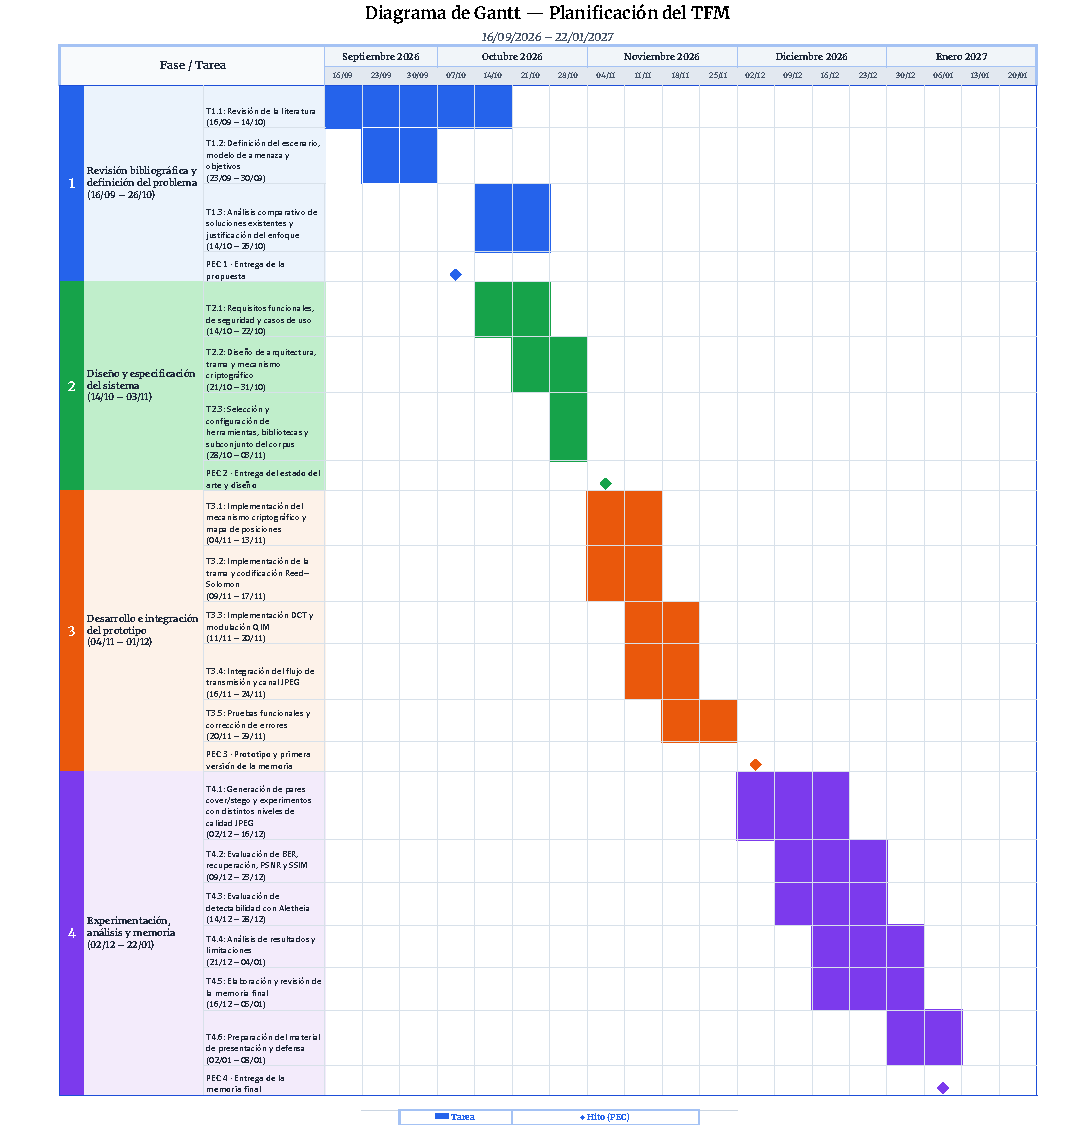
\includegraphics[width=\textwidth]{Imagenes/DG_TFM.pdf}
    \caption{Planificación temporal del TFM}
    \label{fig:gantt_tfm}
\end{figure}

\subsection{Recursos necesarios}

Para ejecutar la planificación definida y desarrollar el prototipo experimental se requiere el uso de los siguientes recursos:

\begin{itemize}

\item \textbf{Recursos de hardware:} Equipo informático personal con arquitectura x64 y al menos 8 GB de memoria RAM, suficiente para la ejecución de los algoritmos de esteganografía, los procesos de codificación y decodificación, las pruebas de compresión JPEG y el cálculo de las métricas de evaluación. No se requiere el uso de una $\mathrm{GPU}$ dedicada.

\item \textbf{Recursos de software:} Entorno de desarrollo basado en Python 3.11, junto con las librerías \texttt{NumPy}, \texttt{OpenCV} y \texttt{Pillow} para el procesamiento y análisis de imágenes, y \texttt{scikit-image} para calcular el $\mathrm{SSIM}$; \texttt{reedsolo} para la aplicación del código Reed--Solomon $RS(8,4)$; y \texttt{cryptography} para implementar el intercambio de claves X25519 y la derivación de claves mediante HKDF. También utilizaremos la suite \texttt{Aletheia} \cite{1} para la evaluación mediante técnicas de estegoanálisis y un sistema de control de versiones para gestionar el desarrollo del prototipo.

\item \textbf{Recursos de datos:} Conjunto de imágenes de prueba obtenido a partir de un subconjunto del corpus ALASKA2, que contiene imágenes en color en formato JPEG. Para los experimentos se utilizarán exclusivamente las imágenes originales (\textit{cover}), descartando las que contienen información esteganográfica (\textit{stego}). Este corpus nos permitirá evaluar el comportamiento del prototipo sobre imágenes con características visuales diversas y estudiar su respuesta ante diferentes condiciones de recompresión JPEG.
\end{itemize}

\subsection{Gestión de riesgos y planes de mitigación}

Identificamos los principales riesgos que podrían afectar a la planificación temporal o al cumplimiento de los objetivos técnicos del proyecto. Para cada uno de ellos establecemos un plan de mitigación que permita reducir su impacto y mantener la viabilidad del trabajo.

\begin{enumerate}

\item \textbf{Riesgo 1: Tasa de error de bit ($\mathrm{BER}$) elevada tras la recompresión JPEG.}
\begin{itemize}
    \item \textit{Impacto:} Alto (dificultad o imposibilidad de recuperar correctamente la trama experimental).
    \item \textit{Plan de mitigación:} Mantendremos fija la redundancia Reed--Solomon $RS(8,4)$ definida en el diseño y ajustaremos el paso de cuantificación ($\Delta$) utilizado por QIM, estudiando su comportamiento frente a distintos niveles de calidad JPEG. Asimismo, analizaremos los coeficientes DCT de frecuencias medias, más estables frente a la cuantificación, y priorizaremos las configuraciones que proporcionen un equilibrio adecuado entre robustez y calidad perceptual.
\end{itemize}

\item \textbf{Riesgo 2: Aumento de la detectabilidad del canal encubierto.}
\begin{itemize}
    \item \textit{Impacto:} Alto (el sistema podría presentar características estadísticas que faciliten la detección del contenido oculto).
    \item \textit{Plan de mitigación:} Analizar distintas configuraciones de incrustación y estudiar el comportamiento de los coeficientes de frecuencias medias utilizados por QIM, buscando un equilibrio entre robustez y modificaciones introducidas en la imagen. Utilizaremos los resultados obtenidos mediante Aletheia para identificar las configuraciones con mayor detectabilidad y descartarlas.
\end{itemize}

\item \textbf{Riesgo 3: Desviación de los plazos durante la implementación del prototipo.}
\begin{itemize}
    \item \textit{Impacto:} Medio (posible retraso en el desarrollo y en las pruebas experimentales).
    \item \textit{Plan de mitigación:} Priorizaremos inicialmente la implementación de un prototipo funcional mínimo y utilizaremos bibliotecas consolidadas para las operaciones criptográficas, el procesamiento de imágenes y la codificación de errores. El desarrollo propio se centrará principalmente en la lógica de incrustación y extracción, la generación del mapa de posiciones y la integración de los distintos componentes.
\end{itemize}

\item \textbf{Riesgo 4: Complejidad en la integración del esquema de esteganografía de clave pública con el sistema de incrustación.}
\begin{itemize}
    \item \textit{Impacto:} Alto (dificultad para completar la implementación del protocolo previsto dentro del plazo establecido).
    \item \textit{Plan de mitigación:} Descomponer el desarrollo en módulos independientes y validar cada componente de forma aislada antes de realizar la integración. En caso de dificultades con la integración completa, priorizaremos una versión experimental mínima que permita comprobar el establecimiento del secreto compartido, la reconstrucción del mapa de posiciones y el funcionamiento de la incrustación y extracción QIM.
\end{itemize}

\end{enumerate}


%\section{Breve sumario de productos obtenidos}

%No hay que entrar en detalle: la descripción detallada se hará en el resto de capítulos.


%\section{Breve descripción de los otros capítulos de la memoria}

%Breve explicación de los contenidos de cada capítulo y su relación con el proyecto global.
% El resto del artículo se organiza de la siguiente manera: La Sección 2 contiene la revisión de la literatura. En la Sección 3 , proponemos enfoques para la incrustación de información eficiente y sin errores en el área DCT de imágenes digitales mediante el método QIM . En la Sección 4 , presentamos un nuevo algoritmo de incrustación basado en los enfoques propuestos . La Sección 5 muestra los resultados de experimentos computacionales con este algoritmo. La Sección 6 incluye una comparación con trabajos previos y un análisis de los resultados. La Sección 7 resume nuestra investigación.

\section{Declaración sobre el uso de inteligencia artificial generativa}

%Explicación de cualquier uso que se haya hecho de herramientas de inteligencia artificial generativa (como ChatGPT, Gemini, DALL-E, u otras) durante la concepción y desarrollo de este Trabajo Final, así como la redacción de esta memoria y la preparación de la presentación. Es obligatorio especificar las herramientas concretas utilizadas, la finalidad (por ejemplo, ideación, esbozo de código, corrección gramatical, generación de imágenes, etc.), los períodos o fases del trabajo en los que se emplearon, las acciones realizadas para validar los contenidos generados mediante IA y una valoración crítica del impacto de su uso. Se debe aclarar explícitamente qué partes del trabajo son autoría íntegra del estudiante y cuáles se han basado en inputs o resultados generados por IA, asegurando en todo momento que la responsabilidad intelectual y la validación final del contenido recaen totalmente en el estudiante, y que su uso ha sido discutido con el tutor/a del Trabajo y se ha realizado acorde a sus indicaciones. 

En cumplimiento de las directrices académicas de la UOC respecto al uso de tecnologías emergentes, detallamos a continuación la utilización de herramientas de Inteligencia Artificial Generativa (IAG) durante la concepción, estructuración y redacción de las fases desarrolladas hasta la presente entrega (PEC 1 y PEC 2):

\begin{itemize}
    \item \textbf{Herramientas utilizadas:} Se han utilizado puntualmente herramientas de Inteligencia Artificial Generativa basadas en modelos de lenguaje (\textit{Large Language Models}), concretamente ChatGPT y Gemini.

    \item \textbf{Finalidad y fases de uso:} La utilización de estas herramientas ha abarcado la fase inicial de planificación (PEC 1) y la elaboración del Estado del Arte y el Diseño del Sistema (PEC 2). Se han empleado como apoyo para el formateo de sintaxis LaTeX, la corrección gramatical y de estilo académico, la estructuración de los apartados, la aclaración de conceptos técnicos y el refinamiento de la redacción formal, especialmente en la especificación del modelo de claves ECDH/KDF y la formulación del plan experimental.

    \item \textbf{Validación del contenido:} Las decisiones metodológicas y de arquitectura del prototipo, entre ellas la delimitación de la carga útil a 32 bits, el esquema de canal $RS(8,4) + \mathrm{QIM\text{-}DCT}$, la derivación de la semilla mediante ECDH+HKDF, la transmisión de la clave pública efímera ($epk_A$) mediante un canal auxiliar y la exclusión de mecanismos de autenticación del emisor, corresponden al autor. La información técnica y las propuestas obtenidas mediante IAG se han revisado y contrastado mediante la consulta de literatura especializada y el análisis crítico de su adecuación al alcance del trabajo.

    \item \textbf{Valoración crítica e impacto:} Las herramientas de IAG han servido como apoyo a las tareas de redacción, maquetación y discusión técnica, facilitando la preparación del documento. La selección de las soluciones adoptadas, su justificación y la responsabilidad sobre el contenido final corresponden al autor.
\end{itemize}

%Se declara de forma explícita que la responsabilidad intelectual, la autoría del diseño propuesto y la validación final de todos los contenidos expresados en este documento recaen íntegramente en el estudiante, habiendo seguido las orientaciones y directrices fijadas para el desarrollo del Trabajo Final de Máster.

\chapter{Estado del arte}
%Estado del arte del tema en cuestión. Tendría que acabar mostrando por qué el trabajo es importante y aporta algo, y con las hipótesis del trabajo.

\section{Fundamentos de Esteganografía en Imágenes y Métricas de Rendimiento}

La protección de la información es uno de los pilares fundamentales de la seguridad informática. Para ello, existen dos disciplinas complementarias que desempeñan un papel importante: la criptografía y la esteganografía \cite{13}. Aunque ambas pueden combinarse para añadir capas de seguridad, en este trabajo nos centramos en la esteganografía aplicada a imágenes. No desarrollaremos primitivas criptográficas propias ni cifraremos el mensaje; únicamente emplearemos primitivas estándar (X25519 y HKDF) para derivar, a partir de las claves del receptor, el mapa secreto de posiciones de inserción. En este paradigma, el mensaje que se desea ocultar se integra en un archivo soporte denominado \textbf{cover} (imagen original) para obtener una \textbf{stego-image} (imagen modificada) con el \textbf{payload} cargado (los datos a transmitir) \cite{3}, siendo el objetivo primordial que las modificaciones resulten imperceptibles a la vista humana e indistinguibles estadísticamente de un archivo convencional.

El rendimiento de un método esteganográfico depende de varios factores \cite{11,3}:

\begin{itemize}
    \item \textbf{Capacidad:} Representa la cantidad de información útil (\textit{payload}) que puede ocultarse dentro del medio portador.
    \item \textbf{Imperceptibilidad:} Mide el grado de distorsión visual introducido en la imagen tras la incrustación, evaluado habitualmente mediante métricas como el \textit{Peak Signal-to-Noise Ratio} ($\mathrm{PSNR}$) y el \textit{Structural Similarity Index Measure} ($\mathrm{SSIM}$).
    \item \textbf{Detectabilidad:} Es la vulnerabilidad del estegosistema frente a herramientas de estegoanálisis estadístico capaces de identificar alteraciones en las distribuciones del cover.
    \item \textbf{Robustez:} Determina la capacidad del mensaje oculto para ser recuperado sin errores tras someter a la \textit{stego-image} a procesamientos de señal o transformaciones con pérdida en el canal, tales como la recompresión JPEG o el filtrado \cite{16}.
\end{itemize}

Estas propiedades mantienen una relación de compromiso (\textit{trade-off}): incrementar la cantidad de información insertada o aplicar modificaciones más intensas para aumentar la robustez ante la recompresión JPEG degrada la calidad visual y puede facilitar la detección de anomalías por un observador.

\subsection{Clasificación según el Dominio de Inserción y Resistencia al Canal}

Los métodos de esteganografía en imágenes digitales pueden clasificarse principalmente según el dominio en el que se realiza la modificación de los datos \cite{3}:

\begin{enumerate}
    \item \textbf{Dominio Espacial:} Las modificaciones se aplican directamente sobre los valores de los píxeles. La técnica más extendida es la sustitución del bit menos significativo (\textit{Least Significant Bit}, LSB). Aunque presentan alta capacidad y baja complejidad computacional, los métodos espaciales son extremadamente frágiles ante cualquier procesamiento de señal o compresión con pérdida.
    \item \textbf{Dominio Frecuencial:} La imagen se transforma previamente a un dominio espectral para modificar sus componentes frecuenciales en lugar de los píxeles directos. Entre las transformadas más extendidas destacan la Transformada Discreta del Coseno (\textit{Discrete Cosine Transform}, DCT), la Transformada Discreta de Fourier (DFT) y la Transformada Discreta Wavelet (\textit{Discrete Wavelet Transform}, DWT) \cite{14}.
\end{enumerate}

La elección del dominio de inserción influye en el comportamiento del sistema frente a las transformaciones que puede sufrir la imagen durante su transmisión. En particular, la recompresión JPEG modifica los coeficientes frecuenciales y puede dificultar la recuperación de la información oculta, especialmente cuando el método de inserción no está diseñado para resistir este tipo de transformación. Por ello, los esquemas robustos suelen incorporar codificación de canal, como los códigos Reed--Solomon (RS) \cite{reed1960,20}. En este contexto, nuestro TFM se centra en la esteganografía de imágenes en el dominio frecuencial, mediante la combinación de la DCT y la modulación por índice de cuantificación (QIM). Nuestro objetivo es estudiar la transmisión de una trama experimental de señalización de 32 bits ($V \parallel T$) y evaluar su recuperación tras aplicar diferentes factores de calidad JPEG, utilizando la tasa de error de bit ($\mathrm{BER}$), métricas de calidad visual y pruebas de detectabilidad. De este modo, pretendemos caracterizar experimentalmente el comportamiento del prototipo, evaluando su respuesta ante distintas condiciones.

\section{Esteganografía en el dominio DCT: propuesta de Soria-Lorente y Berres}

Soria-Lorente y Berres \cite{13} presentaron en 2017 un algoritmo esteganográfico que combina la transformada discreta del coseno ($\mathrm{DCT}$), utilizada en el procesamiento de imágenes JPEG, con una estrategia de selección de bloques basada en su entropía, denominada \textit{Entropy Thresholding}. Su propuesta parte de la idea de que no todos los bloques de una imagen ofrecen las mismas condiciones para ocultar información, por lo que la selección de las posiciones de inserción constituye un aspecto relevante del diseño.

El algoritmo divide la imagen en bloques de $8 \times 8$ píxeles y aplica la DCT a cada uno de ellos. A continuación, calcula la entropía de los bloques transformados y selecciona aquellos cuya entropía supera la media de la imagen. En los bloques seleccionados, los coeficientes se cuantizan y se aplica un recorrido en \textit{zigzag} para organizar sus componentes frecuenciales. La información se inserta en los siete primeros coeficientes $\mathrm{AC}$ considerados por el método, siempre que se cumplan tanto el criterio de entropía como las condiciones establecidas por la secuencia pseudoaleatoria.

La generación de esta secuencia constituye otro elemento relevante de la propuesta. Los autores combinan una clave pública y una clave privada para determinar las posiciones en las que se insertan los bits del mensaje. La modificación de los coeficientes se realiza mediante una regla de sustitución basada en la paridad: los valores resultantes representan el bit que se desea ocultar. Una vez completada la inserción, se aplican las transformaciones inversas para reconstruir la imagen esteganográfica.

En cuanto al mecanismo de claves, podemos diferenciar esta construcción del modelo formal de esteganografía de clave pública propuesto por von Ahn y Hopper \cite{4}. Aunque Soria-Lorente y Berres utilizan las denominaciones de clave pública y privada, su artículo establece que tanto el emisor como el receptor disponen del sistema de claves privadas y que el receptor proporciona su clave pública al emisor. Además, ambos procesos utilizan las dos claves para generar las posiciones de inserción y recuperar el mensaje. Por tanto, el uso de estas denominaciones no basta para atribuir al algoritmo las garantías de seguridad computacional demostradas para las construcciones formales de von Ahn y Hopper \cite{4}.

Para evaluar el método, los autores comparan las imágenes originales y las esteganográficas mediante distintas métricas, entre ellas la relación señal-ruido de pico ($\mathrm{PSNR}$), medidas de diferencia y correlación, análisis de histogramas y entropía relativa. También realizan pruebas de estegoanálisis basadas en el ataque Chi-cuadrado ($\chi^2$). Los resultados presentados muestran una buena calidad visual y una resistencia favorable frente a este ataque en las condiciones experimentales estudiadas. No obstante, estos resultados deben interpretarse dentro del alcance de las pruebas realizadas y no permiten garantizar la indetectabilidad frente a cualquier método de estegoanálisis.

Este trabajo constituye un antecedente relevante para nuestro TFM por la combinación de la DCT con un criterio adaptativo de selección de bloques y por la evaluación conjunta de la calidad visual y determinadas propiedades estadísticas. Sin embargo, nuestra propuesta utiliza la modulación por índice de cuantificación ($\mathrm{QIM}$) como técnica de inserción. Además, nuestro estudio evaluará específicamente la recuperación del mensaje tras la recompresión JPEG aplicada después de generar la imagen esteganográfica. Para ello, mediremos la tasa de error de bit ($\mathrm{BER}$) bajo diferentes factores de calidad JPEG, junto con métricas de distorsión visual como $\mathrm{PSNR}$ y $\mathrm{SSIM}$ y pruebas de detectabilidad mediante \textit{Aletheia}. De esta forma, buscamos caracterizar experimentalmente el comportamiento del prototipo y determinar las condiciones en las que puede recuperarse la información, sin presuponer que ofrece mejores resultados que las propuestas anteriores.


\section{Esteganografía en el dominio DCT: modulación QIM, detectabilidad y robustez ante recompresión}

\subsection{Principios de QIM y adaptaciones para el control de errores y del histograma}
La inserción de información en coeficientes frecuenciales puede introducir modificaciones que afectan tanto a la calidad de la imagen como a la recuperación del mensaje oculto. Por una parte, la modificación de los coeficientes puede alterar las propiedades estadísticas de la imagen y facilitar su detección mediante técnicas de estegoanálisis. Por otra, el propio proceso de inserción y reconstrucción puede provocar errores en los datos recuperados. Por ello, el diseño de métodos esteganográficos en el dominio frecuencial debe tener en cuenta tanto la recuperación correcta del mensaje como las alteraciones introducidas en la imagen.

Para responder a estos desafíos, Chen y Wornell introdujeron en 2001 la modulación por índice de cuantificación (\textit{Quantization Index Modulation}, QIM) como una familia de técnicas de inserción que representa los símbolos mediante conjuntos de cuantificadores disjuntos \cite{11}. La regla de decisión en recepción se basa en identificar la celda de cuantificación a la que pertenece la señal recibida, lo que elimina la interferencia de la propia imagen de cobertura sobre la extracción. Este enfoque proporciona el marco teórico para analizar el compromiso entre la capacidad de carga útil, la distorsión introducida y la tolerancia al ruido \cite{11}. Sin embargo, la formulación original de QIM no constituye por sí misma un esquema de clave pública ni garantiza la recuperación libre de errores tras una recompresión JPEG. Esta limitación justifica en nuestro trabajo la integración de codificación correctora de errores Reed--Solomon y la definición de una lógica asimétrica para la gestión de las claves.

A partir de este marco teórico, diversos autores han propuesto adaptaciones de QIM orientadas a resolver problemas específicos en imágenes digitales. Noda, Niimi y Kawaguchi \cite{15} desarrollaron en 2006 dos variantes de esteganografía JPEG basadas en QIM en el dominio DCT. Su trabajo parte de que una aplicación directa de QIM puede modificar significativamente el histograma de los coeficientes DCT cuantizados, por lo que la primera estrategia busca conservar dicho histograma mediante el uso coordinado de dos cuantificadores, mientras que la segunda persigue una preservación aproximada modificando el proceso tradicional de inserción QIM. Al comparar sus propuestas con el algoritmo F5, los autores muestran que es posible reducir la huella estadística en el histograma manteniendo niveles competitivos de capacidad y calidad visual ($\mathrm{PSNR}$).

Por su parte, Evsutin, Melman y Meshcheryakov \cite{14} aplicaron en 2021 QIM sobre el dominio DCT, identificando como una de las principales dificultades la aparición de errores durante la propia fase de inserción. Estos errores surgen de la pérdida de precisión al reconstruir los valores enteros de los píxeles a partir de los coeficientes frecuenciales modificados. Para corregir este efecto, los autores diseñaron un procedimiento iterativo que verifica y ajusta la inserción hasta asegurar la extracción exacta del mensaje. Además, incorporaron una adaptación de la inserción a las características de cada imagen para enmascarar las distorsiones en el histograma de los coeficientes DCT.

En conjunto, estas adaptaciones muestran que la aplicación de QIM sobre el dominio DCT requiere tratar de forma diferenciada la corrección de errores de redondeo y la preservación de las distribuciones estadísticas. Sin embargo, ni la corrección de errores durante el proceso de inserción ni la conservación del histograma garantizan por sí solas la supervivencia de la trama tras una transformación agresiva del canal. Esta distinción resulta fundamental en el estudio de la recompresión JPEG, donde la modificación de las matrices de cuantificación afecta de forma directa a los coeficientes que albergan la información oculta. Por ello, en nuestro trabajo evaluaremos experimentalmente la degradación de la trama recuperada ($\mathrm{BER}$) frente a distintos factores de calidad $Q$, analizando de forma simultánea la distorsión perceptual ($\mathrm{PSNR}$ y $\mathrm{SSIM}$) y la detectabilidad estadística mediante estegoanálisis.

\subsection{Minimización de la distorsión: la perspectiva de J-UNIWARD}

J-UNIWARD, desarrollado por Holub, Fridrich y Denemark \cite{17}, constituye uno de los referentes fundamentales en la esteganografía adaptativa sobre el dominio JPEG. A diferencia de las técnicas orientadas exclusivamente a la preservación del histograma o a la cuantificación directa, J-UNIWARD basa su diseño en la minimización de una función de distorsión definida sobre las componentes frecuenciales de la imagen. Mediante un banco de filtros direccionales, el algoritmo asigna un coste de modificación a cada coeficiente DCT, priorizando la inserción en regiones complejas o con textura, donde las alteraciones resultan estadísticamente menos detectables frente a herramientas de estegoanálisis basadas en modelos ricos (\textit{rich models}).

Es importante matizar que J-UNIWARD no es un esquema equivalente a la propuesta de este trabajo. Mientras que J-UNIWARD persigue la máxima indetectabilidad en canales sin ruido mediante la selección adaptativa de coeficientes y la minimización de la distorsión, nuestro prototipo se articula alrededor de la modulación QIM, la codificación correctora de errores y la recuperación de la trama tras la recompresión. No obstante, los métodos de esteganografía adaptativa ponen de manifiesto la necesidad de considerar el impacto estadístico de cada modificación y no únicamente su visibilidad perceptual.

\subsection{Robustez ante la recompresión JPEG}
\label{subsec:robustez_jpeg}

El comportamiento de un canal encubierto no solo está condicionado por la imperceptibilidad visual o la seguridad estadística teórica, sino también por la supervivencia de la información tras atravesar canales con pérdida, como los servicios de compartición de imágenes. La literatura sobre esteganografía JPEG robusta señala que estos canales aplican con frecuencia procesos automáticos como el redimensionado, el descarte de metadatos y la recompresión con matrices de cuantificación distintas de las originales \cite{18,20}. Estas operaciones modifican los coeficientes DCT y provocan que los métodos adaptativos diseñados para canales sin ruido, como J-UNIWARD, pierdan la información incrustada si carecen de mecanismos de redundancia o de tolerancia al canal \cite{18}.

\paragraph{Cómo se evalúa la robustez.} En los trabajos revisados, la robustez se mide a dos niveles: a nivel de bit (tasa de error de bit o su complemento, la exactitud de bits) y a nivel de mensaje (tasa de éxito, es decir, proporción de imágenes cuyo mensaje se recupera íntegro tras decodificar el código corrector) \cite{18,20,zhu2018hidden}. Las condiciones del canal se fijan mediante el compresor empleado (por ejemplo, las funciones de MATLAB o la biblioteca mozjpeg \cite{18}) y el factor de calidad $Q$, y los resultados dependen de ambos y del corpus utilizado. Esta es también la lógica de evaluación que seguiremos en nuestro prototipo ($\mathrm{BER}$ y recuperación de la trama frente a $Q$).

\paragraph{Métodos con codificación de canal y modulación por dither.} Zhang et al. \cite{20} parten del marco de esteganografía robusta, es decir, construcción de un dominio resistente a la compresión + códigos RS-STC, que combina un código Reed--Solomon con códigos de trellis de síndromes (STC). Su contribución no es un nuevo método de inserción, sino un análisis de tolerancia a fallos de los métodos que siguen este marco: modelan los errores tras la recompresión como errores en ráfaga mediante una distribución de Poisson, validan el modelo con una prueba $\chi^2$ y obtienen una cota inferior de la probabilidad de que el decodificador RS-STC extraiga correctamente el mensaje, que contrastan con resultados experimentales. Entre los métodos de esta familia figura DMAS \cite{zhang2018dmas}, que modifica coeficientes AC de frecuencias medias mediante modulación con \textit{dither} y emplea RS junto con STC. Esa modulación es una realización práctica de QIM, propuesta por Chen y Wornell \cite{11}. Por tanto, la combinación de una inserción basada en cuantificación con Reed--Solomon no es en sí misma novedosa en la esteganografía JPEG robusta. Lo específico de nuestro prototipo es la configuración: QIM sin STC ni funciones de coste adaptativas, un código fijo $RS(8,4)$ sobre una trama de 32 bits, un mapa de posiciones derivado de $SK_B$ y de información pública del protocolo, y el estudio sistemático del efecto de $\Delta$ sobre $\mathrm{BER}$, $\mathrm{PSNR}$, $\mathrm{SSIM}$ y detectabilidad. Los límites de \cite{20} son que se circunscribe a la recompresión JPEG y a esa familia de métodos, que su resultado es una cota y no una garantía, y que no evalúa la detectabilidad.

\paragraph{Selección de regiones robustas mediante aprendizaje.} Zhang, Zhao y He \cite{18} abordan la robustez desde la elección de la región de inserción: entrenan un clasificador de robustez que predice qué bloques DCT no cambian tras la recompresión, y lo emplean para delimitar el dominio de inserción del mensaje secreto. La información de selección se inserta como mensaje de protocolo en coeficientes de frecuencias medias, protegida con un código Reed--Solomon (símbolos de 8 bits), mientras que el mensaje secreto se codifica con BCH. Evalúan la recompresión con mozjpeg y con MATLAB ($Q$ = 75, 85 y 90) sobre BOSSbase 1.01, miden la tasa de éxito de extracción y la comparan con GMAS y con otros métodos robustos, y evalúan la detectabilidad con DCTR y GFR. Sus resultados indican mayor tasa de éxito que GMAS, pero la seguridad frente a los detectores es mejor que la de GMAS solo con cargas altas, y el clasificador debe ajustarse a cada canal de compresión.

\paragraph{Alternativas aprendidas de extremo a extremo.} HiDDeN \cite{zhu2018hidden} entrena conjuntamente un codificador, un decodificador y un adversario, e intercala entre codificador y decodificador capas de ruido que simulan desenfoque gaussiano, eliminación de píxeles (\textit{dropout}), recorte y compresión JPEG. Como la cuantificación JPEG no es diferenciable, durante el entrenamiento se emplean aproximaciones diferenciables (JPEG-Mask y JPEG-Drop) y la robustez se verifica después con JPEG real. Los autores miden la exactitud de bits sobre imágenes de test no vistas: con JPEG real de $Q=50$, la exactitud pasa del 50\,\% (modelo entrenado sin ruido) al 85\,\% (modelo entrenado con JPEG simulado), y reconocen que en distorsiones del dominio frecuencial su modelo rinde peor que un producto comercial de marcado de agua. Entre sus limitaciones para nuestro contexto destacan que la robustez se limita a las distorsiones incluidas en el entrenamiento, que los mensajes son cortos (30 bits en el experimento de robustez) y que la robustez y el secreto se evalúan en configuraciones distintas: el experimento de esteganografía supone un canal sin ruido, y en él el estegoanalizador ATS \cite{lerch2016ats} detecta las imágenes con un 98\,\% de acierto si conoce los pesos del modelo y no mejor que el azar si no los conoce. StegaStamp \cite{tancik2020stegastamp} extiende la idea a la captura física de imágenes: su canal simulado incluye deformación de perspectiva, desenfoque de movimiento y de enfoque, manipulación de color, ruido y compresión JPEG. Codifica 100 bits que, tras corrección de errores con un código BCH, transportan 56 bits de datos, y sus autores informan de la recuperación de aproximadamente el 95\,\% de los bits en condiciones reales de impresión y captura. Su objetivo es la invisibilidad perceptual para enlazar fotografías con recursos en línea, no la indetectabilidad estadística, y requiere una red adicional de detección y rectificación de la imagen.

\begin{table}[H]
\centering
\scriptsize
\caption{Métodos de esteganografía robusta ante recompresión JPEG: canal considerado, evaluación y limitaciones.}
\label{tab:robustez_metodos}
\begin{tabular}{|p{2.3cm}|p{3.3cm}|p{4.7cm}|p{4.3cm}|}
\hline
\rowcolor{uocnavy}
\color{white}\textbf{Método} &
\color{white}\textbf{Transformaciones del canal} &
\color{white}\textbf{Evaluación de la robustez} &
\color{white}\textbf{Limitaciones} \\
\hline
Zhang et al. (2018) \cite{20} &
Recompresión JPEG (modelo de errores en ráfaga). &
Modelo teórico (Poisson, prueba $\chi^2$) y tasa de extracción correcta tras JPEG comparada con la cota teórica. &
Solo recompresión JPEG y familia RS-STC; la cota no es una garantía; no evalúa detectabilidad. \\
\hline
Zhang et al. (2023) \cite{18} &
Recompresión JPEG (mozjpeg y MATLAB; $Q$ = 75, 85, 90). &
Tasa de éxito de extracción; comparación con GMAS y otros métodos; detectabilidad con DCTR y GFR. &
Clasificador ajustado a cada canal; seguridad mejor que GMAS solo con cargas altas; evaluado sobre BOSSbase. \\
\hline
Zhu et al. (2018), HiDDeN \cite{zhu2018hidden} &
Desenfoque gaussiano, \textit{dropout}, recorte y JPEG (simulado en entrenamiento). &
Exactitud de bits sobre imágenes no vistas; con JPEG real de $Q=50$, 85\,\% tras entrenar con JPEG simulado. &
Robustez limitada a lo visto en entrenamiento; mensajes cortos; robustez y secreto evaluados por separado. \\
\hline
Tancik et al. (2020), StegaStamp \cite{tancik2020stegastamp} &
Perspectiva, desenfoque, color, ruido, JPEG, impresión y captura. &
Recuperación de bits en condiciones reales (cerca del 95\,\% de 100 bits, con BCH). &
Objetivo de invisibilidad perceptual, no de indetectabilidad; requiere detección y rectificación de la imagen. \\
\hline
\end{tabular}
\end{table}

A partir de estos antecedentes, el prototipo no asume que la combinación de QIM y Reed--Solomon constituya una solución óptima, sino que la utiliza como base para evaluar su comportamiento en condiciones de laboratorio reproducibles. Tampoco se compara experimentalmente con las alternativas aprendidas, que exigen entrenamiento y quedan fuera del alcance del trabajo. De este modo, se estudiará la recuperación de la trama sintética de 32 bits ($M = V \parallel T$) y se delimitará el rango de factores de calidad $Q$ en el que el canal encubierto mantiene una recuperación fiable del mensaje.

\subsection{Estegoanálisis y detectabilidad}
\label{subsec:estegoanalisis}

Conviene distinguir con claridad los métodos de inserción de los detectores. J-UNIWARD \cite{17}, los métodos de \cite{18} y \cite{20}, HiDDeN y StegaStamp son técnicas de inserción cuya detectabilidad debe evaluarse; el estegoanálisis, en cambio, es el conjunto de técnicas que intentan decidir si una imagen contiene un mensaje. Los primeros detectores eran específicos de un método o de una propiedad estadística, como el ataque $\chi^2$ empleado en \cite{13} o los ataques basados en histogramas considerados en \cite{15}. Frente a la esteganografía adaptativa se impusieron después detectores generales, basados en características de alta dimensión con un clasificador entrenado, y más recientemente redes profundas:

\begin{itemize}
    \item \textbf{Modelos ricos (\textit{rich models}):} Fridrich y Kodovský \cite{fridrich2012rich} proponen conjuntos de características de alta dimensión calculadas a partir de residuos de la imagen y clasificadas mediante un conjunto de clasificadores; su adaptación a imágenes JPEG se presenta en \cite{kodovsky2012jpegrich}.
    \item \textbf{DCTR y GFR:} Son extractores de características específicos para JPEG. DCTR \cite{holub2015dctr} se basa en histogramas de coeficientes obtenidos con la DCT sin diezmado y destaca por su baja complejidad; GFR \cite{song2015gfr} emplea filtros de Gabor bidimensionales. Ambos se utilizan, por ejemplo, para evaluar la seguridad de la esteganografía JPEG robusta en \cite{18}.
    \item \textbf{Detectores profundos:} SRNet \cite{boroumand2019srnet} es una red residual aplicable tanto a imágenes en el dominio espacial como a JPEG, y trabajos posteriores han adaptado redes preentrenadas en ImageNet al estegoanálisis de imágenes JPEG \cite{yousfi2020imagenet}.
    \item \textbf{Estegoanálisis no supervisado:} ATS \cite{lerch2016ats} genera un conjunto de entrenamiento artificial aplicando repetidamente el algoritmo de inserción a las imágenes bajo análisis; es el estegoanalizador utilizado en \cite{zhu2018hidden} para medir el secreto de HiDDeN.
\end{itemize}

El reto ALASKA2 \cite{cogranne2020alaska2}, de cuyo corpus se extraen las imágenes de este trabajo, se planteó para evaluar el estegoanálisis con imágenes realistas. Aletheia \cite{1} integra en una suite de código abierto extracción de características (SRM, GFR y DCTR), modelos profundos (SRNet y EfficientNet-B0) y simuladores de algoritmos de inserción, por lo que constituye una opción práctica y reproducible para esta evaluación. Los simuladores incluidos corresponden a algoritmos ya existentes y sus modelos están entrenados para métodos y tasas de inserción concretos, de modo que, para evaluar el prototipo, será necesario generar pares \textit{cover}/\textit{stego} con la propia implementación y analizarlos con los detectores disponibles. Como esos detectores no conocen nuestro método, sus resultados son indicativos; entrenar un detector específico sería lo ideal, pero queda fuera del alcance de este trabajo. En nuestro trabajo, estos resultados complementan las métricas de distorsión perceptual y permiten analizar la huella estadística de la modulación QIM. Dado que la detectabilidad depende del detector, de la imagen y de la carga insertada, los resultados deben interpretarse dentro del alcance de los detectores, las imágenes y las condiciones experimentales seleccionadas, y no como una garantía general de indetectabilidad.

\subsection{Software y herramientas existentes}
\label{subsec:software_existente}

Existen herramientas de código abierto que implementan técnicas de esteganografía en JPEG. Entre las clásicas se encuentran Steghide \cite{hetzl2005steghide}, que inserta información en los coeficientes DCT mediante un enfoque basado en grafos, OutGuess \cite{provos2001outguess}, que compensa los cambios para preservar las estadísticas de primer orden, y el algoritmo F5 \cite{westfeld2001f5}, basado en codificación matricial. Estas herramientas se diseñaron para minimizar la detectabilidad y no para tolerar una recompresión posterior, por lo que no incorporan mecanismos de corrección de errores ni de clave pública. En el ámbito del estegoanálisis y la experimentación, Aletheia \cite{1} incluye detectores y simuladores de, entre otros, F5, Steghide, OutGuess y J-UNIWARD, y StegoLab \cite{2} ofrece material y herramientas de referencia. Hasta donde alcanza nuestra revisión, no hemos identificado una herramienta de código abierto que combine los tres elementos del prototipo propuesto: vinculación del mapa de posiciones con una clave pública, inserción QIM-DCT con codificación Reed--Solomon y evaluación conjunta de robustez y detectabilidad. Esta afirmación se limita a las fuentes consultadas.

\section{Esteganografía de clave pública: de los modelos formales a la práctica experimental}
\label{sec:esteganografia_clave_publica}

\subsection{El marco fundacional de von Ahn y Hopper}

La esteganografía de clave pública aborda una limitación estructural de los sistemas esteganográficos convencionales: la necesidad de que emisor y receptor compartan previamente un secreto. Este requisito puede dificultar el establecimiento de una comunicación encubierta cuando ambas partes no han intercambiado ninguna clave con anterioridad.

Para resolver esta restricción, von Ahn y Hopper \cite{4} presentaron en \textit{Public-Key Steganography} (EUROCRYPT 2004) el primer modelo formal de esteganografía de clave pública basado en seguridad computacional. Su trabajo establece las condiciones bajo las cuales es posible construir protocolos esteganográficos seguros sin intercambio previo de claves, siempre que se cumplan determinados supuestos criptográficos.

Los autores parten de la distinción entre la seguridad basada en la teoría de la información y la seguridad computacional. En el esquema estudiado, la esteganografía de clave pública no puede alcanzar seguridad demostrable desde un enfoque teórico-informacional estricto sin un secreto compartido. Por ello, adoptan un modelo computacional que limita las capacidades del adversario a algoritmos probabilísticos de tiempo polinómico ($\mathrm{PPT}$, \textit{Probabilistic Polynomial Time}), exigiendo que un observador no pueda distinguir una comunicación esteganográfica de una ordinaria con una ventaja no despreciable.

Para formalizar este planteamiento, los autores representan el estegosistema de clave pública mediante tres algoritmos:
\begin{equation}
S = (SG, SE, SD)
\end{equation}

\begin{itemize}
    \item \textbf{Generación de claves ($SG$):} El algoritmo $SG(1^k) \rightarrow (PK, SK)$ recibe un parámetro de seguridad $1^k$ y genera el par de claves pública ($PK$) y privada ($SK$) del receptor.
    \item \textbf{Incrustación ($SE$):} Utiliza la clave pública $PK$, el mensaje oculto $m$ y el historial de comunicación $h$ para generar la secuencia esteganográfica, con acceso a un oráculo de muestreo del canal.
    \item \textbf{Extracción ($SD$):} Emplea la clave privada $SK$, la secuencia recibida y el historial $h$ para recuperar el mensaje oculto $m$.
\end{itemize}

A partir de esta formalización, los autores analizan diversos escenarios de ataque, como el de texto oculto elegido (\textit{Chosen Hiddentext Attack}, CHA), e introducen el protocolo de intercambio esteganográfico de claves (\textit{Steganographic Key Exchange Protocol}, SKEP). Asimismo, extienden la seguridad frente a adversarios con acceso a oráculos de extracción en el modelo de oráculo aleatorio (ROM).

\subsection{Extensión del modelo ante adversarios activos: Backes y Cachin}

Backes y Cachin \cite{19} ampliaron en 2005 el marco teórico de von Ahn y Hopper orientando su análisis hacia escenarios con adversarios activos (\textit{active wardens}). En su propuesta, el adversario no se limita a la inspección pasiva del canal, sino que puede realizar consultas adaptativas a un oráculo de extracción.

Los autores formalizan la seguridad esteganográfica frente a ataques de texto cubierto elegido adaptativo (SS-CCA) y una relajación denominada SS-PDR-CCA, nociones estrechamente relacionadas con la seguridad CCA de los criptosistemas de clave pública, y muestran que un estegosistema SS-PDR-CCA puede construirse a partir de un criptosistema PDR-CCA seguro con textos cifrados pseudoaleatorios, para distribuciones de texto cubierto con suficiente min-entropía. Al igual que en la propuesta de von Ahn y Hopper, la construcción opera sobre un \textbf{canal esteganográfico abstracto}, modelado formalmente como una distribución probabilística sobre la que se asume la capacidad de muestrear secuencias válidas.

El análisis conjunto de los marcos teóricos de von Ahn y Hopper \cite{4} y Backes y Cachin \cite{19} nos permite distinguir los supuestos de la criptografía teórica de los condicionantes físicos del procesado de señal:

\begin{itemize}
    \item \textbf{Modelo formal de seguridad:} Ambos trabajos estudian la seguridad esteganográfica frente a adversarios con capacidades computacionales acotadas. Backes y Cachin amplían el modelo al considerar adversarios activos.
    \item \textbf{Mecanismo de claves:} En ambas formalizaciones, el emisor requiere únicamente la clave pública $PK$ del receptor para incrustar el mensaje, mientras que la capacidad de extracción queda reservada al poseedor de la clave privada $SK$.
    \item \textbf{Canal de transporte:} Las dos construcciones asumen un canal abstracto o un oráculo de muestreo idealizado. Ninguno de los dos trabajos analiza contenedores multimedia específicos, ni trabaja con píxeles, coeficientes DCT o bloques de compresión.
    \item \textbf{Robustez práctica:} Ninguno de los modelos formales evalúa empíricamente la recuperación del mensaje tras transformaciones con pérdida, como la recompresión JPEG.
\end{itemize}

Esta comparación muestra que deben tenerse en cuenta dos aspectos diferentes: por un lado, la seguridad del método de ocultación mediante clave pública \cite{19,4} y, por otro, su capacidad para mantener la información oculta cuando la imagen se comprime. Por tanto, un método puede ser seguro y no resistir bien la compresión JPEG, mientras que otro puede soportarla sin garantizar la seguridad de la información oculta. En este trabajo abordamos esta brecha mediante un enfoque dual: tomamos la asimetría de claves de los modelos formales como marco conceptual de seguridad e integramos la modulación QIM-DCT con codificación Reed--Solomon para evaluar la robustez del canal encubierto en condiciones de laboratorio.

\section{Análisis comparativo}

A partir de los trabajos revisados, se distinguen cinco líneas de investigación relacionadas entre sí, pero centradas en aspectos diferentes:

\begin{enumerate}
    \item \textbf{Modelos formales de esteganografía de clave pública \cite{4, 19}:} Establecen las condiciones teóricas de seguridad frente a un adversario, pero operan sobre canales abstractos libres de perturbaciones físicas.
    \item \textbf{Técnicas de inserción en el dominio frecuencial \cite{11, 14, 15, 13}:} Analizan el compromiso entre capacidad, distorsión y preservación estadística (como la modulación QIM en coeficientes DCT), sin proporcionar por sí mismas un esquema asimétrico ni garantizar la supervivencia de los datos ante un canal con pérdida.
    \item \textbf{Esteganografía adaptativa en JPEG \cite{17}:} Minimiza una función de distorsión para reducir la detectabilidad en canales sin ruido.
    \item \textbf{Esteganografía JPEG robusta \cite{20, 18, zhu2018hidden, tancik2020stegastamp}:} Persigue la supervivencia del mensaje tras la compresión, mediante codificación de canal con inserción por cuantificación (familia RS-STC y DMAS), selección de regiones resistentes con clasificadores o redes entrenadas con distorsiones simuladas.
    \item \textbf{Estegoanálisis y evaluación estadística \cite{fridrich2012rich, kodovsky2012jpegrich, holub2015dctr, song2015gfr, boroumand2019srnet, lerch2016ats, 1}:} Examinan si los patrones de modificación alteran la distribución estadística de la imagen hasta hacer detectable el canal encubierto.
\end{enumerate}

Estas propiedades (seguridad con clave pública, robustez ante JPEG y baja detectabilidad) no son equivalentes: mejorar una no garantiza las demás, aunque interactúan entre sí y obligan a un compromiso de diseño. La utilización de un esquema de claves asimétricas no garantiza por sí sola que el mensaje sobreviva a una recompresión JPEG, del mismo modo que la corrección de errores de redondeo durante la inserción no demuestra que la trama se recupere tras un procesamiento agresivo. Asimismo, una elevada calidad perceptual (medida en $\mathrm{PSNR}$ o $\mathrm{SSIM}$) no implica que la modificación resulte indetectable frente a un estegoanálisis avanzado.

La Tabla~\ref{tab:estado_del_arte} sintetiza los trabajos revisados mediante criterios comparables (dominio, uso de clave, resistencia a JPEG, detector empleado y resultados principales) y los contrapone con el alcance del prototipo de este TFM. En ella, «No aplica» indica que el criterio queda fuera del objetivo o del modelo del trabajo, y «No evaluado» que el criterio sería pertinente pero el trabajo no lo contrasta. En concreto, evaluamos el comportamiento de un esquema que combina la selección de posiciones derivada de claves públicas con la modulación $\mathrm{QIM}$ en el dominio $\mathrm{DCT}$ y codificación Reed--Solomon, con el fin de caracterizar experimentalmente el equilibrio entre la recuperación de la información, la calidad visual y la detectabilidad.

\begin{table}[H]
\centering
\scriptsize
\caption{Comparación de técnicas relacionadas y posicionamiento del prototipo propuesto.}
\label{tab:estado_del_arte}
\begin{tabular}{|p{2.1cm}|p{2.2cm}|p{2.1cm}|p{2.5cm}|p{2.3cm}|p{3.2cm}|}
\hline
\rowcolor{uocnavy}
\color{white}\textbf{Referencia} &
\color{white}\textbf{Dominio} &
\color{white}\textbf{Uso de clave} &
\color{white}\textbf{Resistencia a JPEG} &
\color{white}\textbf{Detector empleado} &
\color{white}\textbf{Resultados principales} \\
\hline

Von Ahn y Hopper (2004) \cite{4} &
Canal abstracto (modelo formal). &
Clave pública $PK$ para insertar y privada $SK$ para extraer. &
No aplica (canal idealizado). &
Adversario formal $\mathrm{PPT}$ (no hay detector empírico). &
Seguridad demostrable bajo supuestos criptográficos; ataque de texto oculto elegido. \\
\hline

Backes y Cachin (2005) \cite{19} &
Canal abstracto (modelo formal). &
Clave pública. &
No aplica (canal idealizado). &
Adversario activo formal (SS-CCA, SS-PDR-CCA). &
Nociones de seguridad frente a ataques activos; construcción a partir de criptosistemas PDR-CCA seguros. \\
\hline

Chen y Wornell (2001) \cite{11} &
Inserción genérica por cuantificación (QIM y dither modulation). &
No define esquema de clave pública (considera sistemas de clave privada y sin clave). &
No evaluado con JPEG; análisis teórico frente a ruido gaussiano y ataques acotados. &
No aplica. &
Compromiso teórico entre tasa, distorsión y robustez; combinación con códigos correctores. \\
\hline

Noda et al. (2006) \cite{15} &
Coeficientes DCT cuantizados de JPEG (QIM). &
No aplica. &
No evaluado. &
Ataques basados en histograma. &
Mejor preservación del histograma que F5, con capacidad y $\mathrm{PSNR}$ competitivos. \\
\hline

Evsutin et al. (2021) \cite{14} &
Dominio DCT de imágenes (QIM). &
No aplica. &
No evaluado (corrige errores de inserción, no del canal). &
No especificado. &
Extracción exacta mediante inserción iterativa y adaptación al histograma. \\
\hline

Soria-Lorente y Berres (2017) \cite{13} &
Siete primeros AC de bloques DCT seleccionados por entropía. &
Claves pública y privada usadas por ambas partes (no es esquema formal). &
No evaluado. &
Ataque $\chi^2$. &
Buena calidad ($\mathrm{PSNR}$) y resistencia al ataque $\chi^2$ en sus pruebas. \\
\hline

Holub et al. (2014) \cite{17} &
Coeficientes DCT en JPEG (J-UNIWARD). &
No aplica. &
No evaluado (diseñado para canales sin ruido). &
Rich models y ataques dirigidos. &
Iguala o supera el estado del arte en baja detectabilidad. \\
\hline

Zhang et al. (2018) \cite{20} &
JPEG; familia «dominio resistente + RS-STC» (incluye DMAS, con dither modulation). &
No aplica. &
Sí: modelo de errores en ráfaga tras recompresión. &
No evaluado. &
Cota inferior de la probabilidad de extracción correcta, coherente con los experimentos. \\
\hline

Zhang et al. (2023) \cite{18} &
Bloques DCT de JPEG seleccionados por clasificador; protocolo en frecuencias medias. &
Clave secreta compartida para dividir los bloques. &
Sí: mozjpeg y MATLAB; $Q$ = 75, 85, 90. &
DCTR y GFR. &
Mayor tasa de éxito que GMAS y otros métodos robustos; seguridad mejor que GMAS solo con cargas altas. \\
\hline

Zhu et al. (2018), HiDDeN \cite{zhu2018hidden} &
Redes de extremo a extremo (codificador, decodificador, adversario). &
No aplica. &
Sí: JPEG simulado en entrenamiento; 85\,\% de exactitud de bits con $Q=50$. &
ATS \cite{lerch2016ats} (solo en el experimento sin ruido). &
Robustez frente a varias distorsiones; 98\,\% de detección si se conocen los pesos. \\
\hline

Tancik et al. (2020), StegaStamp \cite{tancik2020stegastamp} &
Redes de extremo a extremo con canal físico simulado. &
No aplica. &
Sí: JPEG y otras distorsiones, impresión y captura. &
No evaluado. &
Cerca del 95\,\% de 100 bits recuperados en condiciones reales (con BCH). \\
\hline

\textbf{Prototipo (TFM)} &
DCT-QIM sobre luminancia $Y$ con $RS(8,4)$. &
Mapa de posiciones derivado de $SK_B$ y de información pública (X25519,HKDF,PRNG). &
Se evaluará la recompresión JPEG con distintos factores de calidad $Q$. &
Aletheia. &
$\mathrm{BER}$ de la trama de 32 bits ($M=V\parallel T$), $\mathrm{PSNR}$, $\mathrm{SSIM}$ y detectabilidad, limitados a las imágenes y detectores evaluados. \\
\hline
\end{tabular}
\end{table}

% 2.3. Codificación de canal para corrección de errores (Reed-Solomon)
% 2.4. Estegoanálisis moderno (Aletheia y clasificadores estadísticos)
% 2.5. Análisis comparativo y Brecha de Investigación (Research Gap)

%\chapter{Análisis de Requisitos y Especificación del Sistema}%Estado del arte del tema en cuestión. Tendría que acabar mostrando por qué el trabajo es importante y aporta algo, y con las hipótesis del trabajo.
\chapter{Arquitectura y Diseño del Prototipo}
\label{chap:diseno_solucion}

En este capítulo definimos el diseño de la solución propuesta y describimos los componentes del prototipo experimental. Partimos de los requisitos y de los objetivos de evaluación para establecer una arquitectura de comunicación entre un emisor y un receptor a través de un canal que puede modificar las imágenes transmitidas, así, la propuesta inserta la información en el dominio frecuencial mediante la Transformada Discreta del Coseno (DCT) y la modulación por índice de cuantificación (QIM), junto con un código corrector de errores Reed-Solomon. Además, incorporamos un mecanismo de clave pública, basado en ECDH sobre X25519, HKDF y un generador pseudoaleatorio (PRNG), que vincula la información del destinatario con la inserción y la extracción. El diseño se orienta a transmitir una trama experimental de 32 bits y a evaluar su recuperación tras la recompresión JPEG. Distinguimos entre las decisiones estructurales del sistema y los parámetros que se concretan durante la implementación, y no damos por cumplidas la recuperación sin errores ni la baja detectabilidad antes de realizar las pruebas.

\section{Requisitos y objetivos de diseño}
\label{sec:requisitos_diseno}

El diseño se apoya en un modelo de amenaza explícito, en requisitos que se pueden verificar y en unos objetivos experimentales que orientan la evaluación práctica.

\subsection{Modelo de amenaza}
\label{subsec:modelo_amenaza}

Mantenemos el modelo del capítulo~1, con \textit{Alice} (emisora), \textit{Bob} (receptor) y un \textit{warden}. Precisamos qué sabe y qué puede hacer este último:

\begin{itemize}
    \item \textbf{Conocimiento.} Conoce el algoritmo y sus parámetros públicos (código $RS(8,4)$, coeficientes utilizados, esquema de derivación). Conoce también la clave pública del receptor ($PK_B$) y la clave pública efímera ($epk_A$). No conoce $SK_B$ ni $esk_A$, por lo que no puede reconstruir el mapa secreto de posiciones.
    \item \textbf{Capacidades.} Como \textit{warden} pasivo, observa las imágenes en tránsito y les aplica técnicas de estegoanálisis. Como \textit{warden} activo, aplica recompresión JPEG con pérdida, con un factor de calidad $Q$ que el emisor desconoce, en el intervalo $50\leq Q\leq 100$.
    \item \textbf{Momento del análisis.} En el escenario principal, el \textit{warden} analiza la imagen tras el canal ($I''$), que es la que llega al receptor. Como referencia, analizamos también la estego-imagen antes del canal ($I'$).
    \item \textbf{Fuera de alcance.} El redimensionado, el recorte, la rotación, el filtrado y cualquier transformación distinta de la recompresión JPEG no se evalúan. Tampoco se contemplan ataques contra el protocolo, como la repetición de mensajes o la suplantación del emisor.
\end{itemize}

\subsection{Requisitos funcionales, de seguridad y no funcionales}
\label{subsec:requisitos_funcionales}

Formulamos los requisitos de modo que cada uno tenga un criterio de verificación. Los valores indicados son criterios de aceptación del prototipo, no resultados ya demostrados.

\begin{table}[H]
\centering
\scriptsize
\caption{Requisitos del prototipo y criterios de verificación.}
\label{tab:requisitos}
\begin{tabular}{|p{1.1cm}|p{7.2cm}|p{6.2cm}|}
\hline
\rowcolor{uocnavy}
\color{white}\textbf{ID} &
\color{white}\textbf{Requisito} &
\color{white}\textbf{Verificación} \\
\hline
RF-1 & Extracción ciega, sin la imagen original. Como Bob no sabe a priori si una imagen lleva señal, la acepta solo si la decodificación RS finaliza sin error y el campo $V$ coincide con el valor esperado $V_{\mathrm{esp}}$. Esto no garantiza integridad ni autenticidad. & Prueba unitaria del criterio de aceptación. \\
\hline
RF-2 & Trama $M$ de 32 bits: versión $V$ (8 bits) y patrón numérico sintético $T$ (24 bits), usado únicamente para comparar bit a bit la trama enviada y la recibida. & Comparación bit a bit en cada ensayo. \\
\hline
RF-3 & El mapa de posiciones se deriva de $PK_B$ y de un par efímero, y se reconstruye con $SK_B$ y $epk_A$ (apartado~\ref{sec:Modelo_Claves}). & RS-1 y RS-3. \\
\hline
RF-4 & Codificación $RS(8,4)$ antes de la inserción, que recupera la trama si el canal altera como máximo dos símbolos por bloque. & Recuperación con 0, 1 y 2 símbolos alterados. \\
\hline
RF-5 & Parámetros de inserción y de recompresión configurables, y un registro estructurado por ejecución. & Mismos parámetros y semillas, mismo registro. \\
\hline
RS-1 & Acceso al mapa: con una clave incorrecta, la $\mathrm{BER}$ antes de la corrección es próxima a 0.5. & Media entre 0.45 y 0.55 y ninguna aceptación en 5000 extracciones. \\
\hline
RS-2 & Falsos positivos: Bob no acepta imágenes sin señal. & Cero aceptaciones en al menos 5000 extracciones (cota $6\cdot10^{-4}$ al 95\,\%). \\
\hline
RS-3 & Reproducibilidad del mapa: con las mismas claves, el mismo mapa; con claves distintas, mapas distintos. & Comparación de mapas en todas las repeticiones. \\
\hline
RS-4 & Ni $esk_A$, ni $SK_B$, ni el secreto compartido ni la semilla se guardan en los registros. & Búsqueda automática en los registros. \\
\hline
RNF-1 & Rendimiento: inserción, canal y extracción de una imagen en menos de 10 s en un equipo sin GPU. & Cronometraje en la prueba piloto. \\
\hline
RNF-2 & Portabilidad: solo Python 3.11 y las bibliotecas indicadas en el capítulo~1, más la suite Aletheia. & Revisión de dependencias. \\
\hline
RNF-3 & Modularidad: emisor, canal y receptor son módulos independientes. & Pruebas unitarias por módulo. \\
\hline
\end{tabular}
\end{table}

\subsection{Casos de uso previstos}
\label{subsec:casos_uso}

\begin{table}[H]
\centering
\scriptsize
\caption{Casos de uso del prototipo.}
\label{tab:casos_uso}
\begin{tabular}{|p{1.1cm}|p{2.2cm}|p{6.4cm}|p{4.9cm}|}
\hline
\rowcolor{uocnavy}
\color{white}\textbf{ID} &
\color{white}\textbf{Actor} &
\color{white}\textbf{Descripción} &
\color{white}\textbf{Resultado verificable} \\
\hline
CU-1 & \textit{Alice} & Genera el par efímero, deriva el mapa, codifica la trama e inserta los 64 bits en la imagen. & Estego-imagen $I'$ y clave $epk_A$; $\mathrm{PSNR}$ y $\mathrm{SSIM}$ registrados. \\
\hline
CU-2 & \textit{Bob} & Con $SK_B$ y $epk_A$, reconstruye el mapa, extrae los bits y decide si acepta la imagen. & Trama aceptada o rechazo, según RF-1. \\
\hline
CU-3 & Investigador & Ejecuta la batería de ensayos variando $Q$ y el paso de cuantificación. & Registro por ejecución con $\mathrm{BER}$ y estado de la decodificación. \\
\hline
CU-4 & \textit{Warden} simulado & Analiza con Aletheia conjuntos de imágenes \textit{cover} y \textit{stego}. & Exactitud o AUC de los detectores. \\
\hline
CU-5 & Investigador & Extrae con una clave incorrecta y sobre imágenes sin señal. & RS-1 y RS-2 comprobados. \\
\hline
\end{tabular}
\end{table}

\subsection{Objetivos y condiciones experimentales}
\label{subsec:objetivos_experimentales}

Para evaluar las capacidades y limitaciones del prototipo establecemos cuatro objetivos experimentales. Los valores indicados son metas de diseño y no resultados demostrados.

\begin{enumerate}
    \item \textbf{Tolerancia al canal JPEG.} Estudiaremos la recuperación de la trama tras recomprimir las estego-imágenes con distintos factores de calidad $Q$, prestando especial atención al intervalo $Q \geq 50$. Mediremos la tasa de error de bit (\textit{Bit Error Rate}, BER) antes de la decodificación Reed-Solomon y la tasa de recuperación de la trama, que cuenta como fallo tanto una decodificación fallida como una falsa corrección. Que la trama se recupere sin errores en las pruebas no implica una garantía para cualquier escenario de compresión.

    \item \textbf{Calidad visual.} Usaremos la relación señal-ruido de pico (PSNR) y el índice de similitud estructural (SSIM) entre la imagen de cubierta y la estego-imagen, con unos valores orientativos de $\mathrm{PSNR}\geq 38\,\mathrm{dB}$ y $\mathrm{SSIM}\geq 0{.}95$. Con solo 64 bits insertados son umbrales holgados (apartado~\ref{subsec:parametros}); los tomamos como referencia y no como garantía de invisibilidad perceptual.

    \item \textbf{Acceso al mapa y falsos positivos.} Comprobaremos que una clave incorrecta produce una BER próxima a 0.5 y que el criterio de aceptación no acepta imágenes sin señal (RS-1 y RS-2).

    \item \textbf{Análisis de la detectabilidad.} Evaluaremos con Aletheia, para los métodos y formatos que admita, si la inserción produce alteraciones identificables. Estudiaremos la hipótesis de que la selección de coeficientes de frecuencia media da un compromiso favorable entre robustez y distorsión. Esa selección no garantiza por sí sola una menor detectabilidad, de modo que interpretaremos los resultados como evidencia limitada a los detectores, las imágenes y las condiciones empleados.
\end{enumerate}

\section{Arquitectura general del sistema}
\label{sec:arquitectura_general}

Concebimos el sistema como un modelo de comunicación digital sobre un canal que puede modificar las imágenes. La arquitectura se organiza en tres bloques.

\subsection{Modelo conceptual de comunicación}
\label{subsec:modelo_comunicacion}

\begin{itemize}
    \item \textbf{Módulo emisor.} Partimos de la imagen original $I$ y de la trama $M$. El emisor genera un par de claves efímero, deriva con HKDF la semilla del mapa de posiciones a partir del secreto compartido con $PK_B$ y codifica la trama con Reed-Solomon. Después inserta los bits codificados mediante QIM en coeficientes DCT seleccionados, en las posiciones que fija el mapa. El resultado es la estego-imagen $I'$; la clave $epk_A$ se entrega por separado.

    \item \textbf{Canal con pérdida.} Representa las transformaciones que puede sufrir la imagen durante su transmisión o almacenamiento. Para estudiar uno de los escenarios principales del trabajo, aplicamos recompresión JPEG con distintos factores de calidad $Q$, y el resultado es una imagen $I''$ cuyos coeficientes pueden diferir de los usados en la inserción. Es la única transformación que evaluamos.

    \item \textbf{Módulo receptor.} Procesa la imagen recibida $I''$ para recuperar la trama. Con su clave privada y la clave pública efímera, reconstruye el mismo mapa de posiciones, extrae los bits, decodifica con Reed-Solomon y aplica el criterio de aceptación. En el entorno experimental, compara además la trama recuperada ($M'$) con la original ($M$).
\end{itemize}

La secuencia se resume en la Figura~\ref{fig:flujo_sistema}.

\begin{figure}[!htbp]
   \centering
   \includegraphics[width=15truecm]{Imagenes/ArqPrttp.drawio.png}
   \caption{Arquitectura general del sistema de transmisión esteganográfica a través del canal con pérdida.}
   \label{fig:flujo_sistema}
\end{figure}

\subsection{Separación entre diseño conceptual y parámetros de implementación}
\label{subsec:diseno_parametros}

Para mantener una arquitectura flexible, distinguimos entre las decisiones que definen el funcionamiento general del sistema y los parámetros que se concretan o ajustan durante la implementación.

\textbf{Decisiones estructurales del diseño:}
\begin{itemize}
    \item Una carga útil de 32 bits, dividida en los campos $V$ (8 bits) y $T$ (24 bits), codificada con $RS(8,4)$ en 64 bits antes de la inserción.
    \item La división de la imagen en bloques de $8\times8$ píxeles para el cálculo de la DCT.
    \item Un mecanismo de acuerdo de claves ECDH sobre X25519, con derivación de la semilla mediante HKDF y un PRNG que determina el mapa de posiciones.
    \item La clave pública efímera $epk_A$ se entrega por un canal auxiliar público y no se inserta en la imagen.
    \item Una arquitectura modular (emisor, canal con pérdida y receptor) y una evaluación en cuatro ejes: tolerancia al canal, calidad visual, acceso al mapa y detectabilidad.
\end{itemize}

\textbf{Decisiones pendientes de concretar:} el paso de cuantificación $\Delta$, dentro del rango del apartado~\ref{subsec:parametros}, y el subconjunto concreto de imágenes del corpus. Esta separación nos permite justificar las configuraciones a medida que avancemos en las pruebas y analizar su efecto sobre la robustez, la calidad visual y la detectabilidad.

\section{Especificación de módulos del prototipo}
\label{sec:especificacion_modulos}

A partir de la arquitectura, especificamos las operaciones de cada módulo y cómo se conectan. Organizamos el procesamiento en tres etapas (inserción, canal con pérdida y recuperación), lo que nos permite probar cada una por separado y registrar los resultados.

\subsection{Regla QIM con \textit{dither}}
\label{subsec:regla_qim}

La idea de QIM es sencilla. Imaginamos el eje de valores de un coeficiente DCT con dos juegos de marcas intercaladas: las del bit 0 y las del bit 1. Las marcas de un mismo juego están separadas una distancia $\Delta$ (el paso de cuantificación) y las de juegos distintos, $\Delta/2$ (Figura~\ref{fig:qim_jpeg}). Para insertar un bit, movemos el coeficiente a la marca más cercana de su juego; para leerlo, miramos de qué juego es la marca más cercana al valor recibido. Si la imagen cambia un poco, por ejemplo por la recompresión, el bit se sigue leyendo bien mientras el coeficiente no se desplace más de $\Delta/4$ \cite{11}.

Hay un detalle más. Todas las marcas se desplazan una cantidad $d\in[0,\Delta)$ pseudoaleatoria que deriva de la clave, de modo que las marcas del bit $b$ están en $d + b\,\Delta/2 + k\,\Delta$, con $k$ entero. Este desplazamiento se conoce como \textit{dither}. Sin él, las marcas del bit 0 estarían siempre en $0, \Delta, 2\Delta,\dots$ y, como casi todos los coeficientes de frecuencia media están muy cerca de cero, cualquier coeficiente sin modificar, o leído con una clave incorrecta, se leería como un 0. Con el desplazamiento secreto, quien no conoce $d$ no sabe dónde están las marcas y lee bits al azar, y la $\mathrm{BER}$ con clave incorrecta ronda 0.5.

\begin{figure}[H]
   \centering
   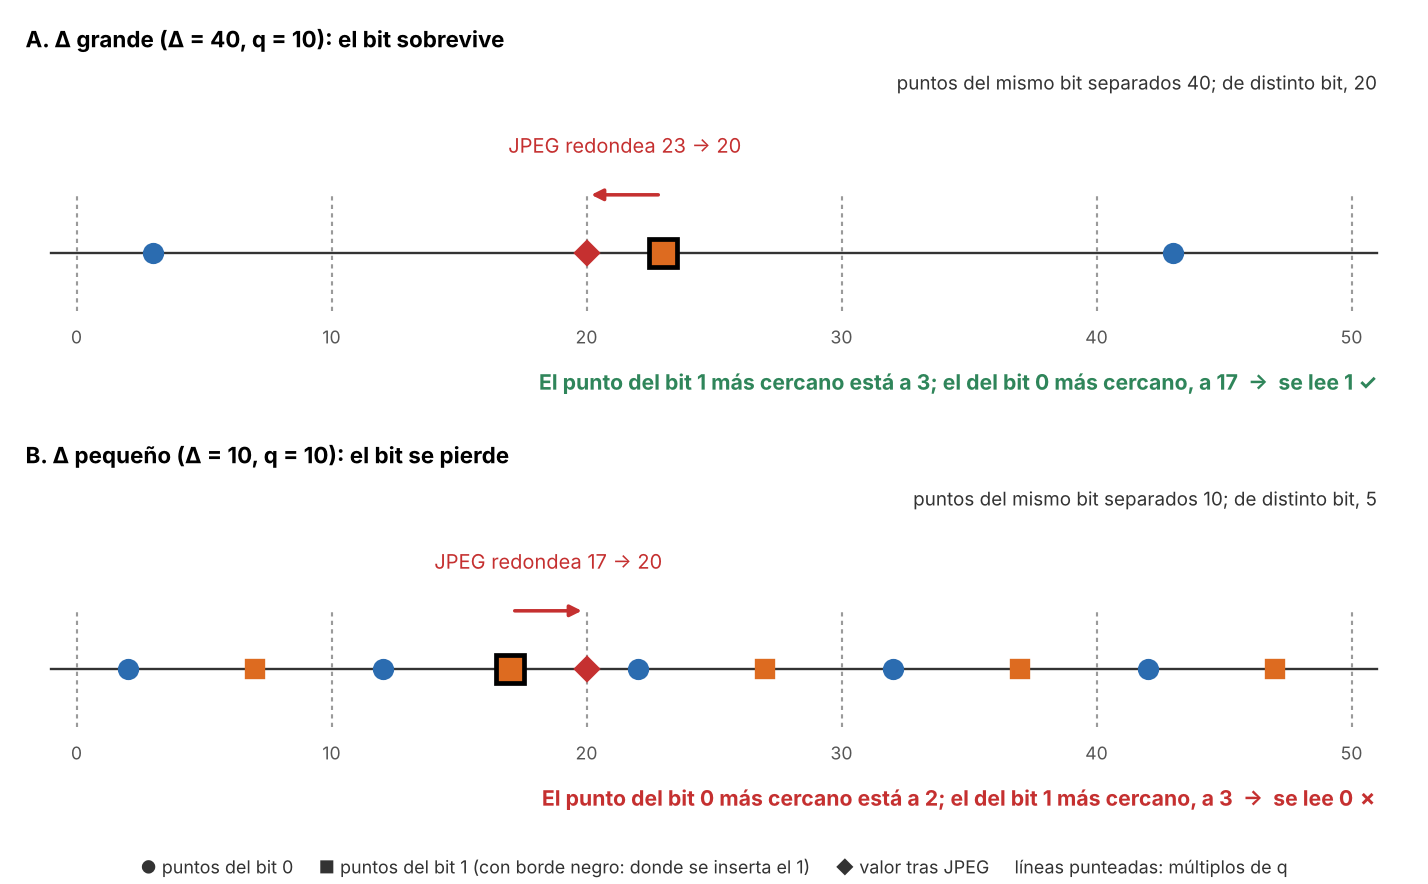
\includegraphics[width=13truecm]{Imagenes/fig_qim_jpeg.png}
   \caption{Ejemplo ilustrativo de QIM con \textit{dither} y recompresión JPEG, con un paso $q=10$ de JPEG. En A, $\Delta=4q$ y el bit sobrevive; en B, $\Delta=q$ y se pierde.}
   \label{fig:qim_jpeg}
\end{figure}

\subsection{Módulo emisor (codificación RS y modulación QIM-DCT)}
\label{subsec:modulo_emisor}

\textbf{Entradas:} imagen original $I$, trama $M$ de 32 bits, clave pública $PK_B$ y paso de cuantificación $\Delta$. \textbf{Salidas:} estego-imagen $I'$ (en PNG, sin pérdidas) y clave pública efímera $epk_A$.

\textbf{Pasos.}
\begin{enumerate}
    \item Generar el par efímero $(esk_A, epk_A)$ y calcular el secreto compartido con $PK_B$.
    \item Derivar con HKDF la semilla e inicializar con ella el PRNG (apartado~\ref{sec:Modelo_Claves}).
    \item Codificar la trama $M$ con $RS(8,4)$: cuatro bytes de datos y cuatro de paridad, es decir, 64 bits.
    \item Obtener la componente de luminancia $Y$ de la imagen y dividirla en bloques de $8\times8$.
    \item Con el PRNG, elegir 64 posiciones distintas (un bloque y un coeficiente del conjunto $\mathcal{C}$ cada una) y los 64 valores de \textit{dither}.
    \item Para cada bloque elegido, calcular la DCT, aplicar la regla QIM a los coeficientes que le corresponden, hacer la DCT inversa, redondear y limitar al intervalo $[0,255]$.
    \item Recomponer la imagen con las componentes $Cb$ y $Cr$ sin modificar y guardarla en un formato sin pérdidas.
\end{enumerate}

\begin{small}
\begin{verbatim}
EMBED(I, M, PK_B, delta):
  (esk, epk) <- X25519.generate();   S <- X25519(esk, PK_B)
  semilla <- HKDF-SHA256(S, contexto || epk || PK_B)
  rng <- PRNG(semilla)
  c <- bits(RS(8,4).encode(M))                  # 64 bits
  Y <- luminancia de I
  P <- 64 pares (bloque, coef.) distintos, elegidos con rng
  d <- 64 valores rng.random() * delta           # dither
  para cada bloque b que aparece en P:
     B <- DCT2(Y[b] - 128)
     para cada i con P[i] = (b, (u,v)):
        D <- delta[u,v];  off <- d[i] + c[i] * D/2
        B[u,v] <- D * round((B[u,v] - off) / D) + off
     Y2[b] <- clip(round(IDCT2(B) + 128), 0, 255)
  I2 <- RGB(Y2, Cb, Cr);  guardar I2 sin perdidas
  return I2, epk
\end{verbatim}
\end{small}

\subsection{Simulación del canal con pérdida (recompresión JPEG)}
\label{subsec:simulacion_canal}

\textbf{Entradas:} estego-imagen $I'$ y factor de calidad $Q$. \textbf{Salida:} imagen recomprimida $I''$.

El módulo de canal recibe la estego-imagen y aplica la recompresión JPEG con el factor de calidad de cada ejecución, introduciendo modificaciones controladas entre la inserción y la extracción. Para cada prueba registramos el factor $Q$ y la configuración del codificador JPEG, y conservamos la imagen resultante. Lo mantenemos independiente del emisor y del receptor, de modo que podamos variar las condiciones de compresión sin tocar los otros módulos y relacionar los resultados con los errores de recuperación.

\subsection{Módulo receptor (extracción QIM y decodificación RS)}
\label{subsec:modulo_receptor}

\textbf{Entradas:} imagen recibida $I''$, clave privada $SK_B$, clave pública efímera $epk_A$ y paso $\Delta$. \textbf{Salidas:} la trama $M'$ aceptada o un rechazo, junto con los 64 bits extraídos y el estado de la decodificación.

\textbf{Pasos.}
\begin{enumerate}
    \item Calcular el secreto compartido con $SK_B$ y $epk_A$, derivar la semilla y reconstruir el mapa de posiciones y los valores de \textit{dither}.
    \item Obtener la luminancia de $I''$, calcular la DCT de los bloques del mapa y aplicar la regla de decisión de QIM a los coeficientes indicados.
    \item Decodificar los 64 bits con Reed-Solomon. Si el decodificador informa de un fallo, rechazar la imagen.
    \item Aceptar la imagen solo si el campo $V$ de la trama decodificada coincide con $V_{\mathrm{esp}}$.
\end{enumerate}

\begin{small}
\begin{verbatim}
EXTRACT(I2, SK_B, PK_B, epk, delta, V_esp):
  S <- X25519(SK_B, epk)
  semilla, rng, P, d <- (igual que en EMBED)
  Y <- luminancia de I2
  para i en 0..63:
     (b,(u,v)) <- P[i];  D <- delta[u,v]
     y <- DCT2(Y[b] - 128)[u,v] - d[i]
     e0 <- |y - D*round(y/D)|
     y1 <- y - D/2;  e1 <- |y1 - D*round(y1/D)|
     c'[i] <- 1 si e1 < e0, si no 0
  intentar M' <- RS(8,4).decode(bytes(c'));  si falla: return RECHAZO
  si M'[0] != V_esp: return RECHAZO
  return ACEPTADA, M'
\end{verbatim}
\end{small}

Una vez finalizado el proceso, comparamos la trama recuperada con la referencia usada en la inserción y registramos por separado los errores de la secuencia extraída, el resultado de la decodificación y la coincidencia final. Distinguimos tres resultados: recuperación correcta, fallo detectado (el decodificador informa de un error) y falsa corrección (el decodificador no informa de error, pero la trama es distinta). Con 64 bits aleatorios, el decodificador $RS(8,4)$, que corrige hasta dos símbolos, devuelve una palabra con probabilidad $\left(1+8\cdot255+28\cdot255^2\right)/2^{32}\approx 4{.}2\cdot10^{-4}$, y con la comprobación de $V$ baja a $\approx 1{.}7\cdot10^{-6}$. Estas cifras suponen lecturas uniformes y las contrastaremos experimentalmente (RS-2).

\subsection{Parámetros de inserción}
\label{subsec:parametros}

\begin{table}[H]
\centering
\scriptsize
\caption{Parámetros de inserción y criterio de elección.}
\label{tab:parametros}
\begin{tabular}{|p{2.6cm}|p{5.0cm}|p{7.4cm}|}
\hline
\rowcolor{uocnavy}
\color{white}\textbf{Parámetro} &
\color{white}\textbf{Valor} &
\color{white}\textbf{Criterio} \\
\hline
Canal de color & Componente $Y$ de YCbCr. & Coherente con el alcance (cap~1); $Cb$ y $Cr$ no se modifican. \\
\hline
Dominio & Bloques de $8\times8$, DCT ortonormal con desplazamiento de 128. & Misma escala que JPEG, de modo que $\Delta$ es comparable con los pasos $q_{u,v}$ de su tabla de cuantificación. \\
\hline
Coeficientes $\mathcal{C}$ & Ocho AC de frecuencia media (índices zigzag 6 a 13), con $q^{(50)}_{u,v}$ entre 13 y 19. & Se excluyen el DC y los AC más bajos (más visibles) y los más altos (cuantificación fuerte). \\
\hline
Actuación de QIM & Coeficientes DCT sin cuantizar, calculados sobre la imagen decodificada. & La recompresión usa otra tabla de cuantificación, así que no se opera sobre los índices cuantizados del JPEG original. \\
\hline
Paso $\Delta_{u,v}$ & $\alpha\,q^{(50)}_{u,v}$, con $\alpha\in\{1{.}5;\,2;\,3;\,4\}$. & Ver el análisis siguiente. \\
\hline
Formato de salida & $I'$ en PNG; $I''$ por recompresión JPEG. & Aísla el efecto del canal y evita una compresión previa de $I'$. \\
\hline
Número de imágenes & 500 \textit{cover} de ALASKA2 \cite{cogranne2020alaska2}. & Imágenes de $512\times512$ en color y JPEG; valor ajustable según el tiempo de cómputo. \\
\hline
\end{tabular}
\end{table}

\textbf{Criterio para $\Delta$.} El paso $\Delta$ de QIM debe ser lo bastante grande para que el redondeo de JPEG no cambie el bit. Lo razonamos en tres pasos:
\begin{enumerate}
    \item JPEG redondea cada coeficiente al múltiplo más cercano de su paso de cuantificación $q$, de modo que lo mueve como mucho $q/2$. Por ejemplo, con $q=13$, un coeficiente de valor 20 pasa a 26, es decir, se mueve 6.
    \item QIM decide bien el bit si el coeficiente se mueve menos de $\Delta/4$ (apartado~\ref{subsec:regla_qim}).
    \item Por tanto necesitamos $q/2<\Delta/4$, es decir, $\Delta>2q$ (Figura~\ref{fig:qim_jpeg}).
\end{enumerate}
Como cada coeficiente tiene su propio paso, definimos $\Delta_{u,v}=\alpha\,q_{u,v}$ y exigimos $\alpha>2$. Además, los pasos $q^{(Q)}_{u,v}$ decrecen al aumentar $Q$, así que un $\Delta$ calculado con la tabla de $Q=50$ sirve también para todo $Q\geq 50$. Los pasos $q^{(50)}_{u,v}$ son los de la tabla de cuantificación de luminancia del estándar JPEG: los ocho coeficientes de $\mathcal{C}$ tienen pasos 16, 14, 13, 14, 18, 17, 16 y 19, es decir, entre 13 y 19. Por eso el rango de $\Delta$ para cada $\alpha$ va de $13\alpha$ a $19\alpha$:

\begin{itemize}
    \item $\alpha=1{.}5$: $\Delta\in[19{.}5;\,28{.}5]$, por debajo del mínimo, para localizar dónde empieza a fallar.
    \item $\alpha=2$: $\Delta\in[26;\,38]$, justo en el límite.
    \item $\alpha=3$: $\Delta\in[39;\,57]$, valor central, con margen frente al ruido de redondeo.
    \item $\alpha=4$: $\Delta\in[52;\,76]$, margen amplio a costa de modificar más la imagen.
\end{itemize}

\textbf{Compatibilidad con $\mathrm{PSNR}\geq 38\,\mathrm{dB}$.} El $\mathrm{PSNR}$ se calcula a partir del error cuadrático medio ($\mathrm{MSE}$) entre las dos imágenes, y para llegar a 38\,dB el $\mathrm{MSE}$ no puede superar $255^2/10^{3{.}8}\approx 10{.}3$, es decir, un error típico de unos 3 niveles de gris por píxel. Nosotros solo modificamos 64 coeficientes en una imagen de $512\times512=262\,144$ valores, y cada uno cambia como mucho $\Delta/2$ (en promedio, su cuadrado es $\Delta^2/12$). Como la DCT ortonormal conserva la energía, ese cambio total se reparte entre todos los píxeles y resulta $\mathrm{MSE}\approx 64\,\Delta^2/(12\cdot 262\,144)$. Con el mayor paso previsto ($\Delta=76$) el $\mathrm{PSNR}$ es de unos 57\,dB, y no se llegaría a 38\,dB hasta $\Delta\approx 712$, casi diez veces más. Por tanto, el $\mathrm{PSNR}$ no limita la elección de $\Delta$ y el compromiso real está entre robustez y detectabilidad. El tamaño de $512\times512$ es el de ALASKA2, y recalcularemos estos valores con el de las imágenes reales.

\subsection{Elección del código corrector}
\label{subsec:eleccion_codigo}

Con posiciones pseudoaleatorias, los errores del canal afectan a bits sueltos, casi independientes entre sí, y un código por bytes como Reed-Solomon pierde su ventaja frente a las ráfagas: $RS(8,4)$ corrige hasta dos símbolos (bytes) erróneos, y tres bits alterados en tres bytes distintos ya lo superan. Un cálculo analítico, suponiendo que cada bit falla con probabilidad $p=0{.}05$, indica que la trama se pierde en el 54\,\% de los casos con $RS(8,4)$, en el 7\,\% con un BCH acortado $(59,32)$ que corrige hasta 5 bits cualesquiera, y en el 21\,\% con repetición triple de los 32 bits. Mantenemos $RS(8,4)$ fijo, conforme al objetivo del trabajo, y tratamos su adecuación como un resultado experimental: registraremos los símbolos y bits erróneos de cada ensayo para comprobar si los errores son independientes o se agrupan. No implementamos BCH ni repetición, y si los errores resultaran independientes, lo discutiremos como una limitación del código elegido.


\section{Modelo de claves}
\label{sec:Modelo_Claves}

Para incorporar la asimetría al prototipo empleamos un acuerdo de claves Diffie--Hellman sobre curva elíptica (ECDH), con la curva X25519 \cite{rfc7748}, y una función de derivación de claves (KDF), concretamente HKDF con SHA-256 \cite{rfc5869}. El objetivo es que emisor y destinatario obtengan un secreto compartido y lo usen para generar de forma determinista el mapa de posiciones, sin necesidad de haber compartido antes una semilla secreta.

El destinatario dispone de un par de claves $(PK_B, SK_B)$: la pública se facilita al emisor y la privada permanece bajo su control. Para cada envío, el emisor genera un par efímero $(epk_A, esk_A)$, y la clave privada $esk_A$ no se transmite. Con claves válidas, ambos obtienen el mismo secreto compartido:
\begin{equation}
S_A = \operatorname{ECDH}(esk_A, PK_B) = \operatorname{ECDH}(SK_B, epk_A) = S_B
\end{equation}
A partir de él, ambos derivan con HKDF la semilla del mapa:
\begin{equation}
K_{\mathrm{mapa}} = \operatorname{HKDF}(S, C)
\end{equation}
donde $C$ es el contexto de derivación, que incluye $epk_A$ y $PK_B$. Esa semilla inicializa el generador de números aleatorios de NumPy (PCG64), que elige sin repetición las 64 posiciones, es decir, los bloques de $8\times8$ y los coeficientes de frecuencia media donde se inserta la trama, y los valores de \textit{dither}. Este generador no es criptográficamente seguro. Lo aceptamos como limitación de un prototipo experimental y lo señalamos como línea de mejora. El destinatario repite la derivación con su clave privada y $epk_A$, y la coincidencia de los mapas depende de que ambos apliquen de forma consistente los mismos parámetros.

La propiedad de seguridad que perseguimos es restringir la reconstrucción del mapa a quien disponga de la clave privada del destinatario, bajo los supuestos criptográficos de ECDH y HKDF. Se refiere al acceso al mapa: no implica indetectabilidad, ni recuperación tras cualquier transformación de la imagen, ni las garantías de un esquema formal de esteganografía de clave pública como el de von Ahn y Hopper \cite{4}. Tampoco hay autenticación del emisor, porque cualquiera que conozca $PK_B$ puede generar su propio par efímero y enviar una señal a Bob, sin que el sistema permita atribuirle un origen. Por eso $M=V\parallel T$ solo se usa para comprobar la recuperación y calcular tasas de error, y no como credencial de identidad.

\subsection{Distribución de la clave pública efímera}
\label{subsec:distribucion_epk}

La clave $epk_A$ debe llegar al destinatario para que pueda calcular el secreto compartido. Descartamos insertarla en la imagen por tres razones:

\begin{itemize}
    \item \textbf{Tamaño.} Una clave X25519 ocupa 256 bits, cuatro veces los 64 bits de la trama codificada, y más si se le añade redundancia. Competiría con la carga útil por la capacidad y aumentaría la detectabilidad.
    \item \textbf{No uniformidad.} Una clave de curva no es una cadena uniforme: es una coordenada de la curva y solo en torno a la mitad de las cadenas posibles corresponden a puntos válidos. Existen codificaciones que lo evitan, como Elligator \cite{bernstein2013elligator}, pero exceden el alcance del prototipo.
    \item \textbf{Comprobación pública.} Si la clave se insertara en posiciones públicas con código corrector, cualquier observador podría extraerla y comprobar si lo leído es una palabra válida, lo que revelaría la presencia de señal.
\end{itemize}

Craver \cite{craver1998} aborda este problema para la esteganografía de clave pública con un \textit{warden} activo: complementa el canal subliminal con un canal supraliminal, cuyo contenido no se oculta pero no puede alterarse sin destruir la imagen, para intercambiar la clave pública. Esta línea queda como trabajo futuro. En el prototipo asumimos, como declaramos en el capítulo~1 (apartado~\ref{subsec:delimitacion_alcance}), que $epk_A$ llega a Bob por un canal auxiliar público, distinto de la imagen. Esto tiene tres consecuencias: el sistema no oculta que existe un intercambio de claves, no evaluamos la recuperación de $epk_A$ y las propiedades que defendemos se limitan al acceso al mapa de posiciones.

\section{Plan de evaluación experimental}
\label{subsec:plan_experimental}

Para responder a los objetivos de la sección~\ref{subsec:objetivos_experimentales}, estructuramos el plan como un procedimiento parametrizable, trazable y reproducible.

\subsubsection{Diseño experimental y variables de control}

Establecemos un entorno de pruebas controlado para evaluar el comportamiento del prototipo ante variaciones en el canal y en los parámetros de inserción:

\begin{itemize}
    \item \textbf{Factor de calidad JPEG ($Q$):} $Q\in\{50, 60, 70, 75, 80, 85, 90, 95, 100\}$. Cubre desde un escenario de compresión relativamente intensa ($Q=50$) hasta la máxima calidad configurada ($Q=100$). Añadimos $Q=60$ porque el salto de 50 a 70 es grande para delimitar un umbral de recuperación. Como la escala de calidad depende del codificador JPEG, registramos el que empleamos.
    \item \textbf{Paso de cuantificación ($\Delta$):} $\Delta_{u,v}=\alpha\,q^{(50)}_{u,v}$, con $\alpha\in\{1{.}5;\,2;\,3;\,4\}$ (apartado~\ref{subsec:parametros}). Estudiaremos su influencia en la distorsión visual y en la recuperación de los bits tras la recompresión.
    \item \textbf{Código corrector:} $RS(8,4)$ sobre $\mathrm{GF}(2^8)$, fijo en toda la evaluación (cuatro bytes de datos, ocho codificados, 64 bits insertados), para estudiar el efecto del canal y de $\Delta$ sin introducir variaciones adicionales en la codificación.
\end{itemize}

\subsubsection{Ejecución de los ensayos}

Seleccionamos 500 imágenes \textit{cover} de ALASKA2 al azar, con una semilla registrada. Para cada imagen y cada valor de $\alpha$ generamos la estego-imagen y la sometemos a cada factor $Q$ de la matriz experimental, lo que da $500\times4\times9=18\,000$ ensayos. En cada uno extraemos con QIM, decodificamos con Reed-Solomon y registramos los errores y el estado de la decodificación, además de las diferencias visuales introducidas. Antes de la batería principal comprobamos que emisor y receptor obtienen mapas coincidentes y que, sin canal, la extracción con la clave correcta recupera todos los bits.

\textbf{Acceso al mapa y falsos positivos.} Como Bob no sabe a priori si una imagen contiene señal, hacemos dos controles. En el primero, extraemos de las estego-imágenes con 10 claves incorrectas por imagen (5000 extracciones) y comprobamos que la $\mathrm{BER}$ antes de la corrección ronda 0.5 y que no se acepta ninguna. En el segundo, aplicamos la extracción sobre imágenes \textit{cover} sin señal, con 10 claves distintas por imagen (5000 extracciones), y contamos cuántas acepta el criterio del receptor.

\textbf{Detectabilidad.} Construimos conjuntos de imágenes \textit{cover} y \textit{stego}, antes del canal y tras recomprimir ambos con la misma $Q$, y los analizamos con los detectores de Aletheia compatibles con el método \cite{1}. Esos modelos están entrenados para métodos y tasas de inserción concretos y no para el nuestro, así que sus resultados, en exactitud o AUC, son solo indicativos. Entrenar un detector con nuestro propio método sería lo ideal, pero queda fuera del alcance del trabajo y lo declaramos como limitación. Un resultado cercano al azar no se interpretará como prueba de indetectabilidad.

\subsubsection{Métricas de evaluación}

\begin{itemize}
    \item \textbf{Distorsión visual ($\mathrm{PSNR}$ y $\mathrm{SSIM}$).} Se comparan la imagen original $I$ y la estego-imagen $I'$ en el dominio espacial. El $\mathrm{PSNR}$ cuantifica la distorsión a partir del error cuadrático medio y el $\mathrm{SSIM}$ estima la similitud estructural. Como $epk_A$ no se inserta, los 64 bits codificados son todos los bits modificados, y las métricas reflejan la carga completa. Ninguna de las dos garantiza imperceptibilidad ni resistencia al estegoanálisis.

    \item \textbf{Fiabilidad del canal ($\mathrm{BER}$ y tasa de recuperación).} La tasa de error de bit antes de la corrección se calcula sobre los 64 bits codificados:
    \begin{equation}
    \mathrm{BER}_{\mathrm{raw}} = \frac{1}{64}\sum_{i=1}^{64}\left( M_{\mathrm{cod}}[i] \oplus M'_{\mathrm{cod}}[i] \right)
    \end{equation}
    donde $\oplus$ es la operación XOR. Cuando la decodificación produce una trama válida de 32 bits, la tasa de error posterior es $\mathrm{BER}_{\mathrm{RS}}=\frac{1}{32}\sum_{j=1}^{32}\left( M[j] \oplus M'[j] \right)$. Como $\mathrm{BER}_{\mathrm{RS}}$ solo existe si hay salida válida, los fallos desaparecerían de su promedio; por eso la métrica principal es la tasa de recuperación sobre $N$ ensayos:
    \begin{equation}
    R = \frac{1}{N}\sum_{k=1}^{N} \left[ M'_k = M_k \right]
    \end{equation}
    En ella, los fallos detectados y las falsas correcciones cuentan como fallos y se informan por separado, y la $\mathrm{BER}_{\mathrm{RS}}$ se informa siempre con su número de casos. Una $R=1$ en una condición de prueba no es una garantía para otras. El código Reed-Solomon opera con símbolos de ocho bits, por lo que su capacidad depende del número de símbolos erróneos y no solo del número de bits alterados; para $RS(8,4)$ es de hasta dos símbolos por bloque.

    \item \textbf{Detectabilidad y acceso al mapa.} Para la detectabilidad, la exactitud o el AUC de los detectores sobre los conjuntos \textit{cover}/\textit{stego}; documentaremos como parte de los resultados las incompatibilidades técnicas y la ausencia de detectores apropiados. Para el acceso al mapa, la media de $\mathrm{BER}_{\mathrm{raw}}$ con clave incorrecta y la tasa de aceptación en los dos controles.
\end{itemize}

\subsubsection{Registro de datos, trazabilidad y reproducibilidad}

Para poder repetir los ensayos, el sistema genera un registro estructurado, en formato JSON o CSV, por cada ejecución. Incluye el identificador y el hash de la imagen, la versión del código, el factor $Q$ y la configuración JPEG, el paso $\Delta$, la configuración RS, el identificador de semilla, $\mathrm{PSNR}$, $\mathrm{SSIM}$, $\mathrm{BER}_{\mathrm{raw}}$, $\mathrm{BER}_{\mathrm{RS}}$, el estado de la decodificación (correcta, fallo o falsa corrección), la decisión de aceptación y el resultado de Aletheia, que se marca como no disponible cuando el detector no puede dar un resultado aplicable. El identificador de semilla remite a la configuración empleada para generar el mapa, sin almacenar el secreto compartido ni otros datos sensibles (RS-4). Con este registro podemos comparar los ensayos bajo distintas condiciones y analizar la relación entre la distorsión visual, la recuperación de la trama y la detectabilidad.


 
\chapter{Implementación y pruebas}
\label{chap:implementacion}

En este capítulo describimos cómo hemos implementado el prototipo diseñado en el capítulo~\ref{chap:diseno_solucion}, es decir, cómo organizamos el código, qué decisiones tomamos en cada módulo 
y con qué pruebas comprobamos que se comporta como esperábamos. Los módulos se explican en el orden en que los hemos desarrollado, de los más sencillos a los que integran todo el flujo.

\section{Entorno y organización del código}
\label{sec:entorno_codigo}

Hemos desarrollado el prototipo en Python 3.11 sobre un equipo personal con Windows, sin GPU, tal como se planificó en el capítulo~1. Las bibliotecas que utilizamos son \texttt{reedsolo} para la codificación Reed-Solomon, \texttt{cryptography} para X25519 y HKDF, \texttt{NumPy} para el generador pseudoaleatorio y la manipulación de bloques, \texttt{OpenCV} y \texttt{Pillow} para el procesamiento de imágenes y la recompresión JPEG, y \texttt{scikit-image} para el cálculo del $\mathrm{SSIM}$. Las versiones exactas quedan registradas en un fichero de requisitos, para que el entorno se pueda reconstruir.
\\
\\
Siguiendo el requisito de modularidad (RNF-3), dividimos el código en módulos independientes, cada uno con una única responsabilidad y con sus propias pruebas unitarias (Tabla~\ref{tab:modulos}). Esta separación nos permite validar cada pieza por separado antes de integrarla con las demás, que era la medida de mitigación prevista para el riesgo de integración (Riesgo~4).

\begin{table}[H]
\centering
\scriptsize
\caption{Módulos del prototipo y estado de la implementación.}
\label{tab:modulos}
\begin{tabular}{|p{2.6cm}|p{7.8cm}|p{3.6cm}|}
\hline
\rowcolor{uocnavy}
\color{white}\textbf{Módulo} &
\color{white}\textbf{Función} &
\color{white}\textbf{Estado} \\
\hline
\texttt{frame.py} & Construir y analizar la trama de 32 bits y convertir entre bytes y bits. & Implementado y probado. \\
\hline
\texttt{coding.py} & Codificar y decodificar con Reed-Solomon $RS(8,4)$. & Implementado y probado. \\
\hline
\texttt{crypto.py} & Generar claves X25519 y derivar la semilla con HKDF. & Implementado y probado. \\
\hline
\texttt{positions.py} & Generar el mapa pseudoaleatorio de posiciones y los valores de \textit{dither}. & Implementado y probado. \\
\hline
\texttt{stego.py} & Insertar y extraer información mediante QIM-DCT. & En desarrollo. \\
\hline
\texttt{channel.py} & Simular la recompresión JPEG. & Pendiente. \\
\hline
\texttt{metrics.py} & Calcular $\mathrm{BER}$, $\mathrm{PSNR}$ y $\mathrm{SSIM}$. & Pendiente. \\
\hline
\texttt{main.py} & Ejecutar el flujo completo con una imagen. & Pendiente. \\
\hline
\end{tabular}
\end{table}

\section{Módulos implementados}
\label{sec:modulos_implementados}

\subsection{Trama experimental}
\label{subsec:impl_frame}

El módulo \texttt{frame.py} construye y analiza la trama $M=V\parallel T$ de 32 bits. Para que emisor y 
receptor interpreten los datos de la misma forma, fijamos tres convenciones: $V$ ocupa el primer byte, los bytes se ordenan en \textit{big-endian} y los bits de cada byte se recorren del más al menos significativo. El valor esperado de $V$ para el criterio de aceptación (RF-1) es una constante del módulo, $V_{\mathrm{esp}}=\texttt{0x01}$, y el patrón $T$ no se escribe a mano: lo genera una función a partir de un generador con semilla registrada, de modo que cada ensayo se puede repetir (RNF-1).
Una decisión que cambiamos durante la implementación afecta a las funciones de conversión entre bytes y bits. 
En las primeras versiones solo aceptaban tramas de 32 bits. Al conectarlas con Reed-Solomon vimos que también debían procesar los 8 bytes, es decir, los 64 bits, de la trama codificada, tanto al insertarla como al reconstruirla en el receptor. Por eso las generalizamos a cualquier longitud múltiplo de 8.

\subsection{Codificación Reed-Solomon}
\label{subsec:impl_coding}

Para $RS(8,4)$, en \texttt{coding.py} utilizamos la biblioteca \texttt{reedsolo} con cuatro símbolos de paridad sobre $\mathrm{GF}(2^8)$: la entrada son cuatro bytes y la salida, ocho. El decodificador puede terminar de dos maneras cuando hay demasiados errores: lanza una excepción, y entonces sabemos que la trama no se ha podido corregir, o devuelve una trama distinta de la original sin avisar, que es lo que llamamos falsa corrección. Mantenemos separados los dos casos porque, en la evaluación, cuentan ambos como fallos de recuperación.

Las pruebas de este módulo comprueban la capacidad correctora del código con todas las combinaciones que interesan: un byte alterado en cada una de las ocho posiciones, las 28 parejas de posiciones (el límite de dos símbolos erróneos), 16 bits alterados concentrados en dos bytes, y tres bits sueltos en tres bytes distintos, que superan la capacidad. Esta última prueba confirma por qué el código pierde ventaja con errores independientes (apartado~\ref{subsec:eleccion_codigo}). Además, contrastamos la probabilidad teórica de falsa corrección: con 100\,000 palabras aleatorias de 8 bytes y una semilla fija, el decodificador aceptó 42, es decir, $4{.}20\cdot10^{-4}$, que coincide con el valor teórico $4{.}2\cdot10^{-4}$ calculado en el diseño.

\subsection{Acuerdo de claves y derivación de laS semilla}
\label{subsec:impl_crypto}

En el módulo \texttt{crypto.py} implementamos el acuerdo de claves con X25519 y la derivación con HKDF-SHA256 de la biblioteca \texttt{cryptography}. Manejamos las claves como bytes en bruto de 32 bytes, sin exponer los objetos de la biblioteca, lo que simplifica las pruebas y el registro de datos. La semilla se deriva con un contexto formado por una etiqueta fija, la clave pública efímera y la clave pública de Bob, como describimos en el apartado~\ref{sec:Modelo_Claves}.

Hay dos decisiones que responden directamente a los requisitos de seguridad. Por un lado, la función del 
emisor devuelve la semilla y la clave pública efímera, pero nunca la privada, de modo que esta no 
puede acabar en un registro (RS-4). Y por otro, una clave pública de orden bajo, por ejemplo 32 ceros, 
se rechaza con un error en lugar de producir un secreto predecible. 

Con las pruebas pudimos comprobar que Alice y Bob  obtienen el mismo secreto y la misma semilla, que cambiar cualquier elemento del contexto cambia la 
semilla, y que una clave privada incorrecta produce otra semilla distinta (base del requisito RS-1).

\subsection{Mapa de posiciones}
\label{subsec:impl_positions}

El módulo \texttt{positions.py} convierte la semilla en el mapa de inserción. Inicializamos con ella el generador
 de NumPy (PCG64), elegimos sin repetición 64 pares (bloque, coeficiente) entre todos los candidatos,
 que son el número de bloques por los ocho coeficientes de frecuencia media, y después generamos los 64 valores de \textit{dither} entre 0 y 1. El orden importa: primero las posiciones y después los \textit{dither}, porque emisor y receptor deben consumir el generador igual para obtener el mismo mapa. El bit $i$ de la trama codificada se inserta en la posición $i$ del mapa. Devolvemos el resultado como tuplas, para que no se pueda modificar por accidente.

La realización de las pruebas dieron un resultado útil en este módulo. La primera versión devolvía enteros de NumPy y no enteros de Python, y la prueba que volcaba el mapa a JSON, el formato del registro de ensayos, falló. Lo corregimos convirtiendo los valores al construir el mapa. Además, comprobamos que la misma semilla da siempre el mismo mapa, que semillas distintas dan mapas distintos y casi sin posiciones en común, y que los valores quedan dentro de rango. Como limitaciones, PCG64 no es criptográficamente seguro, lo que ya aceptamos en el diseño, y NumPy no garantiza secuencias idénticas entre versiones distintas, por lo que fijamos la versión de la biblioteca.

% TODO (PEC 3): ir añadiendo una subsección por módulo conforme se terminen.
% \subsection{Inserción y extracción QIM-DCT}   -> stego
% \subsection{Canal con pérdida}                -> channel
% \subsection{Métricas}                         -> metrics
% \subsection{Flujo completo}                   -> main

\section{Pruebas realizadas}
\label{sec:pruebas}

Cada módulo tiene su propio conjunto de pruebas unitarias, escritas con la biblioteca \texttt{unittest} de Python y ejecutables con un único comando. Las pruebas comprueban cada requisito del apartado~\ref{subsec:requisitos_funcionales} que depende del módulo, y se lanzan completas cada vez que modificamos el código. La Tabla~\ref{tab:pruebas} resume su estado.

\begin{table}[H]
\centering
\scriptsize
\caption{Pruebas unitarias por módulo.}
\label{tab:pruebas}
\begin{tabular}{|p{2.2cm}|p{1.6cm}|p{6.4cm}|p{3.2cm}|}
\hline
\rowcolor{uocnavy}
\color{white}\textbf{Módulo} &
\color{white}\textbf{Pruebas} &
\color{white}\textbf{Qué comprueban} &
\color{white}\textbf{Requisitos} \\
\hline
\texttt{frame} & 11 & Límites de los campos, orden de bytes y de bits, ida y vuelta con 32 y 64 bits, criterio de versión y reproducibilidad de $T$. & RF-1, RF-2, RNF-1 \\
\hline
\texttt{coding} & 9 & Corrección de 1 y 2 símbolos en todas las posiciones, fallo con 3 símbolos y tasa de falsa corrección. & RF-4, RS-2 \\
\hline
\texttt{crypto} & 9 & Simetría del secreto, determinismo de la semilla, dependencia del contexto, claves inválidas y de orden bajo. & RF-3, RS-1, RS-3, RS-4 \\
\hline
\texttt{positions} & 10 & Determinismo, unicidad y rango de las posiciones, entradas inválidas, solapamiento entre semillas y registro en JSON. & RF-3, RS-3 \\
\hline
\end{tabular}
\end{table}

% TODO: actualizar los números de pruebas y añadir las de stego, channel y metrics.
% TODO: añadir la prueba de integración (ida y vuelta sin canal, BER = 0) y el resultado piloto.

% -------------------------------

%\chapter{Resultados}

%Detallad en este apartado los resultados obtenidos utilizando la metodología descrita en el apartado anterior.

%Las figuras tienen que estar explicadas y citadas en el texto, como la \ref{fig:my_label}, en la cual se muestra el error en función de la distancia, en unidades arbitrarias. En todas las gráficas tiene que haber el título de los ejes.

%\begin{figure}[!htbp]
 %   \centering
 %   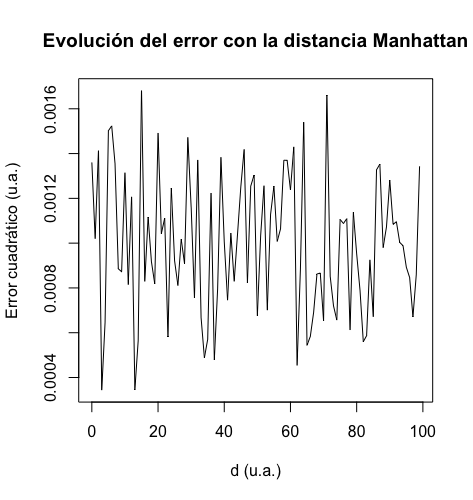
\includegraphics[width=7truecm]{Rplotmanh.png}
 %   \caption{Error en función de la distancia en unidades arbitrarias.}
 %   \label{fig:my_label}
%\end{figure}

%\chapter{Discusión}
%Discusión de los resultados en el contexto del proyecto. Es en este apartado donde cobran sentido y en el cual se responden las preguntas de investigación y se muestra como los resultados dan respuesta a los problemas planteados.

%Esta parte puede ser que no aplique según el tipo de trabajo.

%\chapter{Valoración económica}
%En caso de que corresponda, se incluirá un apartado de ``Valoración económica del trabajo". Este apartado indicará los gastos asociados al desarrollo y mantenimiento del trabajo, así como los beneficios económicos obtenidos. Hay que hacer un análisis final sobre la viabilidad del producto.

%\chapter{Conclusiones y trabajos futuros}

%\section{Conclusiones}
% Este capítulo tiene que incluir:
% \begin{itemize}
% \item Una descripción de las conclusiones del trabajo:
% \begin{itemize}
%     \item Una vez se han obtenido los resultados, ¿qué conclusiones se extraen?
%     \item ¿Estos resultados son los esperados? ¿O han sido sorprendentes? ¿Por qué? 
% \end{itemize}
% \item Una reflexión crítica sobre el logro de los objetivos planteados inicialmente:
% \begin{itemize}
%     \item ¿Hemos logrado todos los objetivos? Si la respuesta es negativa, ¿por qué motivo?
% \end{itemize}
% \item Un análisis crítico del seguimiento de la planificación y metodología a lo largo del producto:
% \begin{itemize}
%     \item ¿Se ha seguido la planificación?
%     \item ¿La metodología prevista ha sido suficientemente adecuada?
%     \item ¿Ha habido que introducir cambios para garantizar el éxito del trabajo? ¿Por qué? 
% \end{itemize}
% \item De los impactos previstos en \ref{s:etic}, ético-sociales, de sostenibilidad y de diversidad, evaluar/mencionar si se han mitigado (si eran negativos) o si se han conseguido (si eran positivos). 
% \item Si han aparecido impactos no previstos a \ref{s:etic}, evaluar/mencionar cómo se han mitigado (si eran negativos) o que han aportado (si eran positivos).
% \item Las líneas de trabajo futuro que no se han podido explorar en este trabajo y han quedado pendientes.


%\item Una descripción de las conclusiones del trabajo: Qué lecciones se han aprendido del trabajo?
%\item Una reflexión crítica sobre el logro de los objetivos planteados inicialmente: Hemos conseguido todos los objetivos? Si la respuesta es negativa, por qué motivo?
%\item De los impactos previstos a la sección \ref{s:etic}, una evaluación, o al menos, mención, sobre si se han mitigado (si eran negativos) o si se han conseguido (si eran positivos). 
%\end{itemize}

%\section{Líneas de futuro}
%Las líneas de trabajo futuro que no se han podido explorar en este trabajo y han quedado pendientes.

%\section{Seguimiento de la planificación}
%Un análisis crítico del seguimiento de la planificación y metodología a lo largo del trabajo: 
%\begin{itemize}
%    \item  Se ha seguido la planificación? 
%    \item La metodología prevista ha sido la adecuada? 
%    \item Ha habido que introducir cambios para garantizar el éxito del trabajo? ¿Por qué? 
%\end{itemize}

% \chapter{Glosario}

% Definición de los términos y acrónimos más relevantes utilizados dentro de la Memoria.


\printbibliography[heading=bibnumbered]




% \newpage
% \appendix
% Listado de apartados que son demasiado extensos para incluir dentro de la memoria y tienen un carácter autocontenido (por ejemplo, manuales de usuario, manuales de instalación, etc.)
 
% Dependiendo del tipo de trabajo, es posible que no haya que añadir algún anexo.



\end{document}
